\documentclass[a4paper, 12pt, oneside, dvipsnames, table]{article}
\usepackage{../../Utilita/Stiletemplate}
\usepackage{hyperref}
\usepackage{fancyhdr}
\usepackage[italian]{babel}
\usepackage[utf8]{inputenc}
\usepackage{float}
\usepackage{siunitx}
\restylefloat{table}

\newcommand{\Data}{2021\_01\_30}

\newcommand{\Titolo}{Verbale riunione \Data}

\newcommand{\Redattori}{\TL}

\newcommand{\Verificatori}{\PC}

\newcommand{\Approvatore}{\VD}

\newcommand{\Distribuzione}{\VT{} \newline \CR{} \newline Gruppo \Gruppo}

\newcommand{\Uso}{Interno}

\newcommand{\DescrizioneDoc}{Questo documento si occupa di riportare quanto discusso nella riunione del \Data.}

\newcommand{\pathimg}{../../../Immagini/N.O.S.jpg}

\newcommand{\Versionedoc}{1.0}
% info generali 
\newcommand{\NomeProgetto}{\textit{Emporio$\lambda$ambda}}

% fornitore
\newcommand{\Gruppo}{\textit{N.O.S}}
\newcommand{\Mail}{nos.unipd@gmail.com}

% committenti
\newcommand{\Committente}{\VT \newline \CR}
\newcommand{\VT}{Prof. Vardanega Tullio}
\newcommand{\CR}{Prof. Cardin Riccardo}

% proponenti
\newcommand{\Proponente}{\textit{RedBabel}}

% Componenti
\newcommand{\BL}{Brescanzin Lorenzo}
\newcommand{\FF}{Fantinato Filippo}
\newcommand{\MM}{Martini Matteo}
\newcommand{\PC}{Panighel Cristiano}
\newcommand{\TG}{Terrani Giulia}
\newcommand{\TL}{Tredese Leonardo}
\newcommand{\VD}{Varotto Davide}

% ruoli

\newcommand{\Responsabile}{\textit {Responsabile di Progetto}}
\newcommand{\Amministratore}{\textit{Amministratore di Progetto}}

% documenti

\newcommand{\SdF}{Studio di Fattibilità}
\newcommand{\SdFv}[1]{\textit{Studio di Fattibilità {#1}}}
\newcommand{\PdQ}{Piano di Qualifica}
\newcommand{\PdQv}[1]{\textit{Piano di Qualifica {#1}}}
\newcommand{\PdP}{Piano di Progetto}
\newcommand{\PdPv}[1]{\textit{Piano di Progetto {#1}}}
\newcommand{\NdP}{Norme di Progetto}
\newcommand{\NdPv}[1]{\textit{Norme di Progetto {#1}}}
\newcommand{\AdR}{Analisi dei Requisiti}
\newcommand{\AdRv}[1]{\textit{Analisi dei Requisiti {#1}}}
\newcommand{\Glossario}{Glossario}
\newcommand{\Glossariov}[1]{\textit{Glossario {#1}}}

% comandi generali
\newcommand{\glo}[1]{#1\ap{G}}

\newcommand{\myparagraph}[1]{\paragraph{#1}\mbox{}\\}

\setcounter{tocdepth}{5}  \setcounter{secnumdepth}{5}


\begin{document}

\copertina{}
\newpage


\fancydoc{}

\registroModifiche{
	
	2.0 & 2021\_03\_06 & \VD{} & Responsabile & - & Approvazione del documento. \\
	
	1.20 & 2021\_03\_05 & \MM{} & Analista & \TL{} & Inseriti UML corretti. \\
	
	1.19 & 2021\_03\_04 & \PC{} & Analista & \TL{} & Aggiornata sezione \S\ref{Tracciamento}. \\
	
	1.18 & 2021\_03\_02 & \PC{} & Analista & \BL{} & Aggiornata sezione \S\ref{ReqFunz}, requisiti del venditore. \\
	
	1.17 & 2021\_03\_01 & \MM{} & Analista & \PC{} & Aggiornata sezione \S\ref{ReqFunz}, requisiti dell'acquirente. \\
	
	1.16 & 2021\_02\_26 & \BL{} & Analista & \PC{} & Correzione dei precedenti e aggiunta di nuovi UC, estensioni di UC già presenti. \\

	1.15 & 2021\_02\_25 & \TG{} & Analista & \PC{} & Correzione UC "Lista riepilogo ordini" ora UC\ref{visualizzazione-ordini-in-gestione} e aggiunta UC da UC\ref{modifica-stato-ordine} a UC\ref{filtro-ordini-venditore}. \\
	
	1.14 & 2021\_02\_24 & \TG{} & Analista & \FF{} & Redatti nuovi UC\ref{ricerca-codice-ordine-acquirente} e UC\ref{filtro-temporale-ordini-acquirente}.\\
	
	1.13 & 2021\_02\_21 & \TG{} & Analista & \FF{} & Redatti nuovi UC\ref{inserimento-indirizzo-consegna}, UC\ref{modifica-indirizzo-consegna} e UC\ref{eliminazione-indirizzo-consegna}. \\
	
	1.12 & 2021\_02\_19 & \MM{} & Analista & \TG{} & Eliminato UC23-"Inserimento campo dati" e UC15-"Modifica informazioni profilo" ora suddiviso in UC\ref{modifica-informazioni-acquirente} e UC\ref{modifica-informazioni-venditore}. \\

	1.11 & 2021\_02\_18 & \PC{} & Analista & \BL{} & Correzione UC\ref{checkout}. \\

	1.10 & 2021\_02\_15 & \BL{} & Analista & \PC{} & Correzioni \S\ref{ReqVincolo} e \S\ref{ReqQual}, da UC\ref{aggiunta-carrello-plp} a UC\ref{modifica-quantita-nel-carrello}.\\
	
	1.9 & 2021\_02\_14 & \BL{} & Analista & \TG & Sistemazione UC\ref{logout} e UC\ref{ricerca-prodotti-acquirente}. \\
	
	1.8 & 2021\_02\_13 & \TG{} & Analista & \MM{} & Aggiunto i casi d'uso UC\ref{aggiunta-categoria}, UC\ref{modifica-categoria}, UC\ref{eliminazione-categoria}. \\

	1.7 & 2021\_02\_10 & \PC{} & Analista & \MM{} & Corretto i caso d'uso UC\ref{aggiunta-prodotto-evidenza} e UC\ref{rimozione-prodotto-evidenza}. \\

	1.6 & 2021\_02\_09 & \TG{} & Analista & \TL{} & Corretto le sezioni UC\ref{aggiunta-prodotto} e UC\ref{modifica-prodotto}. \\
	
	1.5 & 2021\_02\_08 & \MM{} & Analista & \FF{} & Trasformato sottocasi d'uso indipendenti relativi al venditore in casi d'uso. \\
	
	1.4 & 2021\_02\_04 & \MM{} & Analista & \PC{} & Trasformato sottocasi d'uso indipendenti relativi all'acquirente in casi d'uso. \\

	1.3 & 2021\_02\_03 & \TG{} & Analista & \TG{} & Rimossi i dettagli implementativi dai casi d'uso. Eliminato UC3-"Accesso al menù". \\

	1.2 & 2021\_02\_02 & \PC{} & Analista & \TL{} & Separati i casi di accesso alla piattaforma sezione \S\ref{AccessoPiattaforma}. \\

	1.1 & 2021\_02\_02 & \BL{} & Analista & \FF{} & Rimosso l'attore amministratore sezione \S\ref{Attori}. \\ 

	1.0.0 & 2021\_01\_10 & \PC{} & Responsabile & - & Approvazione del documento. \\
	
	0.1.7 & 2021\_01\_09 & \FF{} & Analista & \TL{} & Stesura riepilogo tracciamento \S\ref{Riepilogo} \\
	
	0.1.6 & 2021\_01\_09 & \TL{} & Analista & \BL{} & Stesura tracciamento requisito-fonte \S\ref{ReqFonte} \\
	
	0.1.5 & 2021\_01\_09 & \BL{} & Analista & \FF{} & Stesura tracciamento fonte-requisito \S\ref{FonteReq} \\
	
	0.1.4 & 2021\_01\_08 & \MM{} & Analista & \BL{} & Aggiunta diagrammi dei casi d'uso \S\ref{CasiUso} \\
	
	0.1.3 & 2021\_01\_08 & \TL{} & Analista & \TG{} & Stesura requisiti vincolo \S\ref{ReqVincolo} e prestazionali \S\ref{ReqPrest} \\
	
	0.1.2 & 2021\_01\_08 & \FF{} & Analista & \TG{} & Stesura requisiti di qualità \S\ref{ReqQual} \\
	
	0.1.1 & 2021\_01\_07 & \BL{} & Analista & \TG{} & Stesura requisiti funzionali \S\ref{ReqFunz} \\
	
	0.1.0 & 2021\_01\_06 & - & - & \TG{} & Verifica complessiva del documento. \\
	
	0.0.10  & 2020\_12\_27 & \FF{} & Analista & \TG{} & Stesura caso d'uso UC\ref{estensione:limite-foto-raggiunto}, UC\ref{estensione:prezzo-minore-o-uguale-zero}, UC\ref{estensione:email-non-esistente}, UC\ref{estensione:registrazione-con-email-non-esistente}, UC\ref{estensione:quantita-da-aggiungere-al-carrello-non-valida}, UC\ref{estensione:sconto-minore-zero}, UC\ref{estensione:pagamento-fallito}, UC\ref{estensione:sconto-maggiore-cento} \\
	
	0.0.9 & 2021\_01\_05 & \BL{} & Analista & \TG{} & Stesura casi d'uso: UC\ref{estensione:cambio-con-email-esistente}, UC\ref{estensione:campo-obbligatorio-non-inserito}, UC\ref{estensione:credenziali-non-presenti}, UC\ref{estensione:email-non-valida}, UC\ref{estensione:file-no-tipo-immagine} \\
	
	0.0.8 & 2021\_01\_04 & \TL{} & Analista & \TG{} & Aggiornamento sezioni UC\ref{eliminazione-prodotto}, UC\ref{aggiunta-prodotto-evidenza}, UC\ref{rimozione-prodotto-evidenza}, UC\ref{rifornimento-prodotto} \\
	
	0.0.7 & 2021\_01\_04 & \TL{} & Analista & \TG{} & Aggiornamento sezioni UC\ref{modifica-informazioni-venditore}, UC\ref{eliminazione-account-acquirente}, UC\ref{aggiunta-prodotto}, UC\ref{modifica-prodotto} e \S\ref{Attori} \\
	
	0.0.6 & 2021\_01\_03 & \BL{} & Analista & \TG{} & Stesura casi d'uso: UC\ref{modifica-quantita-da-aggiungere-al-carrello}, UC\ref{eliminazione-prodotto-dal-carrello}, UC\ref{checkout}, UC\ref{visualizzazione-ordini-effettuati}, UC\ref{modifica-informazioni-acquirente} \\
	
	0.0.5  & 2021\_01\_02 & \BL{} & Analista & \TG{} & Stesura casi d'uso: UC\ref{ordinamento-prezzo-decrescente}, UC\ref{aggiunta-carrello-pdp}, UC\ref{aggiunta-carrello-plp} \\
	
	0.0.4  & 2021\_01\_02 & \FF{} & Analista & \TG{} & Stesura casi d'uso: UC\ref{logout}, UC\ref{ricerca-prodotti-acquirente}, UC\ref{filtro-prodotti-acquirente}, UC\ref{ordinamento-prezzo-crescente} \\
	
	0.0.3  & 2021\_01\_01 & \FF{} & Analista & \TG{} & Stesura casi d'uso: UC\ref{registrazione}, UC\ref{autenticazione-acquirente}, UC\ref{autenticazione-venditore}, UC\ref{password-dimenticata} \\ 
	
	0.0.2  & 2020\_12\_27 & \TG{} & Analista & \TL{} & Stesura \S\ref{Desc} \\  
	
	0.0.1  & 2020\_12\_22 & \TG{} & Analista & \BL{} & Stesura scheletro del documento, \S\ref{Intro}, \S\ref{Desc} \\
}

\setcounter{table}{0}

\clearpage
\tableofcontents
\clearpage

\newpage
\listoftables
\newpage
\listoffigures
\newpage

\section{Introduzione}
\subsection{Scopo del Documento}
Questo documento contiene la stesura dello studio di fattibilità riguardante i sette capitolati proposti, elencando quelli che il nostro gruppo ha considerato come i loro aspetti più interessanti e le loro criticità. Infine, per ogni capitolato vengono esposte le motivazioni e le ragioni per cui il gruppo ha scelto come progetto il capitolato C2 \NomeProgetto{} a discapito degli altri sei proposti.

\subsection{Glossario}
Al fine di evitare ambiguità fra i termini, e per avere le terminologie chiare fra tutti gli stakeholder, il gruppo \Gruppo{} ha redatto un documento denominato \Glossariov{1.0.0}.
In tale documento sono presenti tutti i termini tecnici, ambigui, specifici del progetto e scelti dai membri del gruppo con le loro relative definizioni.
Un termine presente nel \Glossariov{1.0.0} e utilizzato in questo documento viene indicato con un apice \ap{G} alla fine della parola.

\subsection{Riferimenti}

\subsubsection{Normativi}
\begin{itemize}
\item \NdPv{1.0.0}.
\end{itemize}

\subsubsection{Informativi}

\begin{itemize}
\item \textbf {Capitolato d'appalto C1 - BlockCOVID:}\\
\url{https://www.math.unipd.it/~tullio/IS-1/2020/Progetto/C1.pdf}
\item \textbf {Capitolato d'appalto C2 - \NomeProgetto:}\\
\url{https://www.math.unipd.it/~tullio/IS-1/2020/Progetto/C2.pdf}
\item \textbf {Capitolato d'appalto C3 - Gathering Detection Platform:}\\
\url{https://www.math.unipd.it/~tullio/IS-1/2020/Progetto/C3.pdf}
\item \textbf {Capitolato d'appalto C4 - HD Viz:}\\
\url{https://www.math.unipd.it/~tullio/IS-1/2020/Progetto/C4.pdf}
\item \textbf {Capitolato d'appalto C5 - PORTACS:}\\
\url{https://www.math.unipd.it/~tullio/IS-1/2020/Progetto/C5.pdf}
\item \textbf {Capitolato d'appalto C6 - Realtime Gaming Platform:}\\
\url{https://www.math.unipd.it/~tullio/IS-1/2020/Progetto/C6.pdf}
\item \textbf {Capitolato d'appalto C7 - SSD:}\\
\url{https://www.math.unipd.it/~tullio/IS-1/2020/Progetto/C7.pdf}

\end{itemize}
\newpage

\section{Analisi dei rischi}
\label{analisi_dei_rischi}
Durante lo sviluppo di un progetto così complesso e di grandi dimensioni, la possibilità di incontrare delle problematiche è alta. Per cercare di evitare il più possibile queste criticità si è svolta un'attenta analisi sui possibili rischi del progetto. La procedura utilizzata per l'analisi dei rischi si suddivide nelle seguenti parti:
\begin{itemize}
    \item \textbf{Individuazione:} \glo{Attività} iniziale di identificazione di possibili problematiche che potrebbero interferire e minare il corretto avanzamento del progetto;
    \item \textbf{Analisi:} Attività di analisi dei singoli rischi con l'obiettivo di evidenziare la probabilità di occorrenza, l'indice di gravità e le conseguenze che  questi potrebbero causare;
    \item \textbf{Pianificazione di Controllo:} Attività di pianificazione delle misure da adottare per cercare di impedire il verificarsi di tali rischi o per gestirli al meglio qualora si verifichino;
    \item \textbf{Monitoraggio:} Attività di controllo costante con lo scopo di evitare il verificarsi di problematiche e permettere di attuare le strategie di contenimento individuate dal gruppo di lavoro per limitarne i danni.
\end{itemize}

Abbiamo suddiviso i principali fattori di rischio nelle seguenti categorie:
\begin{itemize}
    \item \textbf{Rischi legati alle tecnologie;}
    \item \textbf{Rischi legati ai membri del gruppo;}
    \item \textbf{Rischi legati agli strumenti;}
    \item \textbf{Rischi legati all'organizzazione del lavoro;}
    \item \textbf{Rischi legati ai requisiti.}
\end{itemize}

\rowcolors{2}{white}{celeste}
\renewcommand{\arraystretch}{1.5}
\section{Tecnologie, framework e librerie impiegate}
Di seguito vengono descritte tecnologie, framework e servizi di terze parti utilizzati per il progetto.
\subsection{Swagger}
Swagger è un linguaggio di descrizione dell'interfaccia per descrivere le API RESTful espresse utilizzando JSON. Swagger viene utilizzato insieme a una serie di strumenti software open source per progettare, creare, documentare e utilizzare i servizi Web RESTful.
\subsection{AWS Cognito}
AWS Cognito fornisce autenticazione, autorizzazione e gestione degli utenti per le applicazioni Web e mobili. Gli utenti possono accedere direttamente con un nome utente e una password, oppure tramite terze parti, ad esempio Facebook, Amazon, Google o Apple.
I due componenti principali di Amazon Cognito da utilizzare separatamente o insieme sono i pool di utenti, directory utente che forniscono opzioni di registrazione e di accesso, e i pool di identità che consentono di concedere agli utenti l'accesso ad altri servizi AWS.
\subsection{AWS DynamoDB} 
Amazon DynamoDB è un database NoSQL che offre prestazioni veloci e predicibili, in particolare si tratta di un database completamente gestito che consente di scaricare gli oneri amministrativi legati al funzionamento e al ridimensionamento di un database distribuito in modo da non doversi preoccupare del provisioning, dell'installazione e della configurazione dell'hardware, della replica, delle patch del software o del ridimensionamento del cluster eliminando il carico operativo e la complessità coinvolti nella protezione dei dati sensibili. 

\subsection{AWS API Gateway}
Amazon API Gateway semplifica per gli sviluppatori la creazione, la pubblicazione, la manutenzione, il monitoraggio e la protezione delle API RESTful su qualsiasi scala. Le API fungono da “porta di entrata” per consentire l’accesso delle applicazioni ai dati, alla logica aziendale o alle funzionalità dai servizi back-end. 
API Gateway gestisce tutte le attività di accettazione ed elaborazione relative a centinaia di migliaia di chiamate API simultanee, inclusi gestione del traffico, controllo di accessi e autorizzazioni, monitoraggio e gestione delle versioni delle API. 

\subsection{AWS Lambda}
AWS Lambda è un servizio di elaborazione serverless che permette di eseguire il codice senza effettuare il provisioning o gestire i server, creare una logica di dimensionamento dei cluster in funzione dei carichi di lavoro, mantenere integrazioni degli eventi o gestire i runtime. Con Lambda è possibile eseguire codice per qualsiasi tipo di applicazione o servizio di back-end, senza alcuna amministrazione.  È possibile scrivere le funzioni Lambda nel linguaggio preferiro (Node.js, Python, Go, Java e altri ancora) e utilizzare strumenti sia serverless sia di container, come AWS SAM o Docker CLI, per creare, testare e distribuire le funzioni.
\subsection{Amazon S3 Bucket}
È un servizio di storage di oggetti che offre scalabilità, disponibilità dei dati, sicurezza e prestazioni all'avanguardia nel settore offrendo caratteristiche di gestione semplici da utilizzare che consentono di organizzare i dati e di configurare controlli di accesso ottimizzati per soddisfare requisiti aziendali, di pianificazione e di conformità specifici.
\subsection{Amazon SNS}
Amazon Simple Notification Service (Amazon SNS) è un servizio di messaggistica completamente gestito per la comunicazione application-to-person (A2P) e application-to-application (A2A).
Le comunicazioni avvengono in modo asincrono, con un punto di accesso logico e un canale di comunicazione. 
\subsection{Amazon SQS}
Amazon Simple Queue Service (SQS) è un servizio di accodamento messaggi completamente gestito che consente la separazione e la scalabilità di microservizi, sistemi distribuiti e applicazioni serverless. Con SQS, è possibile inviare, memorizzare e ricevere qualsiasi volume di messaggi tra componenti software senza perdite e senza dover impiegare altri servizi per mantenere la disponibilità. 
SQS offre due tipi di code di messaggi: le code standard offrono throughput massimo, ordinamento semplificato e distribuzione di tipo at-least-once mentre le code FIFO sono progettate per garantire che i messaggi vengano elaborati esattamente una sola volta, nell'ordine in cui sono inviati.
\subsection{Stripe}
Stripe è una piattaforma esterna per i pagamenti online che consente all'e-commerce di accettare pagamenti con bancomat, carta ricaricabile o carta di credito. È una soluzione sicura e rapida, i pagamenti vengono elaborati utilizzando strumenti ad hoc sviluppati per la gestione dei flussi di pagamento con controlli anti-frode.
\subsection{NodeJs}
Node.js è un runtime system open source multipiattaforma orientato agli eventi per l'esecuzione di codice JavaScript, ha un'architettura orientata agli eventi che rende possibile l’I/O asincrono. Questo design punta ad ottimizzare il Throughput e la scalabilità nelle applicazioni web con molte operazioni di input/output. Il modello di networking su cui si basa Node.js è I/O event-driven: ciò vuol dire che Node richiede al sistema operativo di ricevere notifiche al verificarsi di determinati eventi, e rimane quindi in sleep fino alla notifica stessa: solo in tale momento torna attivo per eseguire le istruzioni previste nella funzione di callback, così chiamata perché da eseguire una volta ricevuta la notifica che il risultato dell'elaborazione del sistema operativo è disponibile.
\subsection{Npm}
Npm è un package manager per il linguaggio di programmazione JavaScript, il predefinito per l'ambiente di runtime JavaScript Node.js. Consiste in un client da linea di comando, chiamato anch'esso npm, e un database online di moduli pubblici e privati che offrono diverse funzionalità: dalla gestione dell’upload di file, ai database MySQL o a Redis, attraverso framework, sistemi di template e la gestione della comunicazione in tempo reale con i visitatori.
\subsection{TypeScript}
TypeScript è un linguaggio di programmazione open source sviluppato da Microsoft che estende la sintassi di JavaScript, aggiungendo o rendendo più flessibili e potenti varie sue caratteristiche, in modo che qualunque programma scritto in JavaScript sia anche in grado di funzionare con TypeScript senza nessuna modifica. 
\subsection{Next.js}
Next.js è un framework JavaScript back-end per applicazioni React che non richiede alcun setup e che consente il rendering automatico lato server (SSR, server side rendering).
Con Next.js si possono sviluppare applicazioni web, app mobile, desktop e web app progressive: è costruito secondo il principio di “Build once, run anywhere“.
Altre caratteristiche di Next.js sono suddivisione automatica del codice, routing automatico, hot code reloading (viene ricaricato solo il codice modificato) ed esportazione statica (con un solo comando può esportare un sito statico).
\subsection{Jest.js}
Jest.js è un framework di test JavaScript con particolare attenzione alla semplicità e al supporto per applicazioni web di grandi dimensioni.  Fornisce diverse funzionalità come la creazione automatizzata di mock, l'esecuzione di test in parallelo per aumentarne la velocità e la possibilità di testare il codice asincrono in modo sincrono. Jest trova automaticamente i test da eseguire nel codice sorgente, e funziona su progetti JS che includono React, Babel, TypeScript, Node, Angular, Vue.
\subsection{ESLint}
ESLint è uno strumento di analisi del codice statico per identificare pattern problematici o codice che non rispetta certe linee guida predefinite nel codice JavaScript senza eseguirlo. Le regole in ESLint sono configurabili e le regole personalizzate possono essere definite e caricate. ESLint è scritto usando Node.js per fornire un ambiente a runtime veloce e di facile installazione attraverso npm.
\subsection{Material-UI}
Material-UI è una libreria di componenti React per sviluppare il design del proprio progetto o per poter utilizzare tutta una serie di componenti stabili predefiniti.
\subsection{Serverless Framework}
Serverless Framework è un framework Web gratuito e open source scritto utilizzando Node.js, sviluppato per la creazione di applicazioni su AWS Lambda. Il Serverless Framework è costituito da una CLI open source e da una dashboard che insieme, forniscono una gestione completa del ciclo di vita delle applicazioni serverless.

\newpage

\subsection{Rischi legati ai membri del gruppo}


    \begin{table}[H]
        \begin{tabular}{|c|p{10cm}|}
        \hline
        \rowcolor{darkblue}
        \multicolumn{2}{|c|}{\textcolor{white}{\textbf{RG1 - Contrasti tra i Componenti}}} \\
        \hline
         Descrizione & Il gruppo deve cooperare con professionalità nonostante la poca esperienza e non si conoscessero in precedenza, questo può causare tensioni o contrasti.\\ 
         \hline
         Conseguenze & Tensioni o contrasti rallentano e danneggiano il corretto svolgimento del progetto.\\
         \hline
         Probabilità di Occorrenza & Bassa.\\
         \hline
         Pericolosità & Alta.\\
         \hline
         Precauzioni & Ogni elemento del gruppo cercherà di limitare eventuali tensioni a favore del collettivo.\\
         \hline
         Piano di Contingenza & Il {\Responsabile} riassegnerà i compiti per limitare la vicinanza delle parti interessate, eventualmente insieme al resto del \glo{team} cercherà di sanare le incomprensioni.  In casi estremi verrà chiamato in causa il \VT.\\ 
         \hline
        \end{tabular}
        \caption{\label{tab:RG1}Analisi dei rischi per contrasti tra i componenti.}
    \end{table}


    \begin{table}[H]
        \begin{tabular}{|c|p{10cm}|}
        \hline
        \rowcolor{darkblue}
        \multicolumn{2}{|c|}{\textcolor{white}{\textbf{RG2 - Disponibilità dei Membri}}} \\
        \hline
         Descrizione & Ogni membro ha impegni universitari e personali oltre all’attività di progetto; possono inoltre insorgere problemi di salute e familiari che potrebbero rendere i membri improduttivi per alcuni periodi.\\ 
         \hline
         Conseguenze & Possibilità di ritardi su attività individuali o collettive.\\
         \hline
         Probabilità di Occorrenza & Media.\\
         \hline
         Pericolosità & Medio-Alta.\\
         \hline
         Precauzioni & Ogni membro del gruppo è tenuto a compilare un calendario condiviso e deve far presente agli altri componenti del team di eventuali periodi di improduttività. Il {\Responsabile} è così in grado di organizzare al meglio il lavoro.\\
         \hline
         Piano di Contingenza & In caso di mancanze prolungate che provocherebbero pesanti ritardi, il {\Responsabile} si occuperà di ridistribuire i compiti da svolgere ai restanti membri del gruppo di lavoro.\\ 
         \hline
        \end{tabular}
        \caption{\label{tab:RG2}Analisi dei rischi per disponibilità dei membri.}
    \end{table}


    \begin{table}[H]
        \begin{tabular}{|c|p{10cm}|}
        \hline
        \rowcolor{darkblue}
        \multicolumn{2}{|c|}{\textcolor{white}{\textbf{RG3 - Inesperienza Gestionale}}} \\
        \hline
         Descrizione & Il team non ha mai affrontato un progetto di tali dimensioni, nè a livello di carico di lavoro nè per grandezza del gruppo di lavoro. Inoltre, ciascun componente del gruppo non ha esperienza di lavoro che richieda il coordinamento di un gruppo di sette o più persone.\\ 
         \hline
         Conseguenze & Ogni singolo membro del team è disabituato a relazionarsi con un gruppo di persone. I membri del gruppo non hanno familiarità con i ruoli che devono impersonare e con i compiti che devono svolgere portando così possibili ritardi nello sviluppo del prodotto.\\
         \hline
         Probabilità di Occorrenza & Alta.\\
         \hline
         Pericolosità & Alta.\\
         \hline
         Precauzioni & Una frequente comunicazione interna di eventuali difficoltà, specialmente rivolta al {\Responsabile}, aiuterà a mitigare l'insorgere di problemi.\\
         \hline
         Piano di Contingenza & Qualunque difficoltà sarà notificata al {\Responsabile} e affrontata con la collaborazione di tutti. Il {\Responsabile} riassegnerà ai membri più in difficoltà dei compiti  più adatti alle loro competenze. Il componente in questione dovrà eseguire un’autoanalisi per comprendere le motivazioni dei suoi problemi e come migliorare.\\ 
         \hline
        \end{tabular}
        \caption{\label{tab:RG3}Analisi dei rischi per inesperienza gestionale.}
    \end{table}

    \begin{table}[H]
        \begin{tabular}{|c|p{10cm}|}
        \hline
        \rowcolor{darkblue}
        \multicolumn{2}{|c|}{\textcolor{white}{\textbf{RG4 - Scarsa Comunicazione}}} \\
        \hline
         Descrizione & Ciascun membro del gruppo non ha molta esperienza nel \glo{teamwork}, questo può portare a una cattiva comunicazione tra i membri del gruppo.\\ 
         \hline
         Conseguenze & Un'insufficiente comunicazione tra i membri del gruppo può portare a ritardi nello sviluppo del progetto o addirittura a contrasti tra i componeneti stessi.\\
         \hline
         Probabilità di Occorrenza & Bassa.\\
         \hline
         Pericolosità & Media.\\
         \hline
         Precauzioni & Il {\Responsabile} provvederà a monitorare e promuovere un adeguato livello di comunicazione attiva all'interno del team. Non dovranno insorgere situazioni dove, per mancata o scarsa comunicazione, ci siano ritardi nelle decisioni progettuali importanti  con una conseguente insorgenza di situazioni di tensione.\\
         \hline
         Piano di Contingenza & Nel caso si rilevi una scarsa comunicazione da parte di un membro del gruppo sarà compito del {\Responsabile} ricercarne il motivo, se questo si dimostra non lecito provvederà prima ad un richiamo informale (a voce o con gli strumenti di comunicazione interni). Se il comportamento venisse reiterato il {\Responsabile} programmerà una riunione interna al gruppo per discutere la situazione.\\ 
         \hline
        \end{tabular}
        \caption{\label{tab:RG4}Analisi dei rischi per scarsa comunicazione.}
    \end{table}
\newpage

\subsection{Rischi legati agli strumenti}
\newpage

\subsection{Rischi legati all'orgranizzazione}

\begin{table}[H]
    \begin{tabular}{|c | p{10cm}|}
    \hline
    \rowcolor{darkblue}
    \multicolumn{2}{|c|}{\textcolor{white}{\textbf{RO1 - Costi delle Attività}}} \\
    \hline
    Descrizione & Data l'inesperienza del team nella pianificazione di progetto e la messa in pratica della stessa su un arco di tempo medio-lungo, può verificarsi una sottostima o una sovrastima dei costi e dei tempi necessari alla realizzazione del progetto.\\ 
    \hline
    Conseguenze & Una sottostima provocherebbe ritardi nella pianificazione; una sovrastima porterebbe ad uno spreco di tempo. Entrambi i casi richiederebbero poi una nuova pianificazione delle attività.\\
    \hline
    Probabilità di Occorrenza & Medio-Alta.\\
    \hline
    Pericolosità & Alta.\\
    \hline
    Precauzioni & Ogni componente del gruppo controllerà periodicamente lo stato della propria attività rispetto alla tabella di marcia imposta nel documento \textit{\PdP}.\\ 
    \hline
    Piano di Contingenza & Per ogni attività è previsto un tempo di \glo{slack}, in modo da arginare il più possibile il ritardo nell'avanzamento del progetto.\\ 
    \hline
    \end{tabular}
    \caption{\label{tab:RO1}Analisi dei rischi per i costi delle attività.}
    
\end{table}
\newpage

\section{Requisiti}

\subsection{Introduzione}
In questa parte, vengono riportati i requisiti del progetto, classificati per tipologia. Ciascun requisito possiede un codice identificativo, il cui formalismo viene riportato all'interno del documento \NdPv{1.0.0}.

\subsection{Requisiti funzionali} \label{ReqFunz}
\rowcolors{2}{white}{celeste} 
\renewcommand{\arraystretch}{1.5}

\addcontentsline{lot}{table}{Requisiti funzionali}

\begin{longtable}{c C{9.5cm} C{2.5cm}} 

	\rowcolor{darkblue}
	\textcolor{white}{\textbf{Codice Requisito}}&
	\textcolor{white}{\textbf{Descrizione}}&
    \textcolor{white}{\textbf{Fonte}} \\
    
    % Acquirente
    \input{Sezioni/Requisiti/Funzionali/RequisitiAccessoAllaPiattaforma}

    \input{Sezioni/Requisiti/Funzionali/RequisitiAcquirente/RequisitiRicercaDeiProdotti}

    \input{Sezioni/Requisiti/Funzionali/RequisitiAcquirente/RequisitiPLP}

    \input{Sezioni/Requisiti/Funzionali/RequisitiAcquirente/RequisitiPDP}

    \input{Sezioni/Requisiti/Funzionali/RequisitiAcquirente/RequisitiCarrello}

    \input{Sezioni/Requisiti/Funzionali/RequisitiAcquirente/RequisitiCheckout}

    \input{Sezioni/Requisiti/Funzionali/RequisitiAcquirente/RequisitiOrdini}

    \input{Sezioni/Requisiti/Funzionali/RequisitiAcquirente/RequisitiGestioneAccountAcquirente}

    \input{Sezioni/Requisiti/Funzionali/RequisitiAcquirente/RequisitiHome}

    % Venditore
    \input{Sezioni/Requisiti/Funzionali/RequisitiVenditore/RequisitiGestioneAccountVenditore}
    
    \input{Sezioni/Requisiti/Funzionali/RequisitiVenditore/RequisitiProdotto}
    
    \input{Sezioni/Requisiti/Funzionali/RequisitiVenditore/RequisitiRicercaDeiProdottiVenditore}
    
    \input{Sezioni/Requisiti/Funzionali/RequisitiVenditore/RequisitiCategoria}
    
    \input{Sezioni/Requisiti/Funzionali/RequisitiVenditore/RequisitiGestioneOrdini}

\end{longtable}


\subsection{Requisiti di \glo{qualità}} \label{ReqQual}
\rowcolors{2}{white}{celeste} 
\renewcommand{\arraystretch}{1.5}

\addcontentsline{lot}{table}{Requisiti di qualità}

\begin{longtable}{c C{9.5cm} C{2.5cm}} 
	
	\rowcolor{darkblue}
	\textcolor{white}{\textbf{Codice Requisito}}&
	\textcolor{white}{\textbf{Descrizione}}&
	\textcolor{white}{\textbf{Fonte}}\\

	\rqua{O} & La piattaforma deve essere rilasciata sotto \glo{licenza MIT}. & Capitolato  \\

	\rqua{O} & La piattaforma dovrà rispettare la validazione \glo{W3C}. & Interna \\
	
	\rqua{O} & Deve essere realizzata e consegnata una documentazione delle \glo{API} realizzata automaticamente. & VE\_2020\_12\_28 \\
	
	\rqua{O} & La documentazione delle API deve essere scritta in lingua inglese. & VE\_2020\_12\_28 \\
	
	\rqua{D} & È desiderabile avere anche lo stadio di \glo{Production}. & Capitolato \\
	
\end{longtable}


\subsection{Requisiti di vincolo} \label{ReqVincolo}
\rowcolors{2}{white}{celeste} 
\renewcommand{\arraystretch}{1.5}

\addcontentsline{lot}{table}{Requisiti di vincolo}

\begin{longtable}{c C{9.5cm} C{2.5cm}} 
	
	\rowcolor{darkblue}
	\textcolor{white}{\textbf{Codice Requisito}}&
	\textcolor{white}{\textbf{Descrizione}}&
	\textcolor{white}{\textbf{Fonte}}\\

	\rvin{O} & Utilizzo di \glo{Typescript} come principale linguaggio di sviluppo. & \glo{Capitolato} \\
	
	\rvin{O} & Uso del \glo{framework} \glo{Serverless} per il controllo centrale dell'applicazione. & Capitolato \\
	
	\rvin{O} & Le componenti dell'applicazione devono fornire API basata su \glo{HTTP} o \glo{HTTPS}. & Capitolato \\
	
	\rvin{O} & La piattaforma dovrà essere distribuita su \glo{AWS} utilizzando \glo{AWS Lambda} come unità di calcolo. & Capitolato \\
	
	\rvin{O} & La piattaforma va sviluppata con un'architettura a \glo{microservizi}. & Capitolato \\
	
	\rvin{O} & Il \glo{front end} va sviluppato con \glo{Next.js}. & Capitolato \\
	
	\rvin{O} & Il \glo{front end} deve prevedere il pre-rendering della pagina \glo{HTML5} implementato attraverso uno dei due seguenti approcci: \glo{SSR} o \glo{SSG}. & Capitolato \\
	
	\rvin{O} & La piattaforma dovrà integrarsi con il servizio di pagamento Stripe. & Capitolato \\
	
	\rvin{O} & La parte di monitoraggio e controllo della piattaforma \glo{Amazon CloudWatch}. & Capitolato \\
	
	\rvin{Z} & E' necessario memorizzare le credenziali dell'utente su \glo{Auth0}, un \glo{identity provider} esterno di terze parti, per poter migrare il sito da un'infrastruttura all'altra. & Capitolato \\
	
	\rvin{O} & La piattaforma deve essere sviluppata nei seguenti 3 ambienti secondo l'ordine indicato: prima \glo{Locale}, poi \glo{Testing} e dopo \glo{Staging}. & Capitolato \\

	\rvin{O} & La piattaforma deve funzionare correttamente nel browser Google Chrome per desktop dalla versione 88.0.4324.182 in poi. & Interna \\

	\rvin{O} & La piattaforma deve funzionare correttamente nel browser Mozilla Firefox per desktop dalla versione 86.0.0 in poi. & Interna \\

	\rvin{O} & La piattaforma deve funzionare correttamente nel browser Microsoft Edge per desktop dalla versione 88.0.705.68 in poi. & Interna \\

	\rvin{O} & La piattaforma deve funzionare correttamente nel browser Safari per desktop dalla versione 14.0.2 in poi. & Interna \\

	\rvin{O} & La piattaforma deve funzionare correttamente nel browser Google Chrome per mobile dalla versione 88.0.4324.181 in poi. & Interna \\

	\rvin{O} & La piattaforma deve funzionare correttamente nel browser Mozilla Firefox per mobile dalla versione 86.1.1 in poi. & Interna \\

	\rvin{O} & La piattaforma deve funzionare correttamente nel browser Microsoft Edge per mobile dalla versione 46.01.4.5140 in poi. & Interna \\

	\rvin{O} & La piattaforma deve funzionare correttamente nel browser Safari per mobile dalla versione 14.4 in poi. & Interna \\
	
	\rvin{D} & È desiderabile avere anche lo stadio di \glo{Production}. & Capitolato \\
	
\end{longtable}


\subsection{Requisiti prestazionali} \label{ReqPrest}
\rowcolors{2}{white}{celeste} 
\renewcommand{\arraystretch}{1.5}

\addcontentsline{lot}{table}{Requisiti prestazionali}


\begin{longtable}{c C{9.5cm} C{2.5cm}} 
	
	\rowcolor{darkblue}
	\textcolor{white}{\textbf{Codice Requisito}}&
	\textcolor{white}{\textbf{Descrizione}}&
	\textcolor{white}{\textbf{Fonte}}\\

	\rpre{O} & Tempo di riposta di tutte le pagine, escluso il pagamento, sotto i 10 secondi. & Interna \\

\end{longtable}


\newpage

\newpage

\section{Modello di Sviluppo}
\label{modello_di_sviluppo}
Dopo un'attenta lettura del \glo{capitolato} che ha evidenziato la natura a \glo{microservizi} del progetto e dopo una discussione con \Proponente, il gruppo \Gruppo\ ha deciso di adottare, relativamente al ciclo di vita del software, il \textit{modello incrementale} in modo da garantire la qualità e la conformità del prodotto grazie alle maggiori possibilità di poter avere riscontri da parte del proponente. 

\subsection{Modello Incrementale}

\begin{figure}[ht]
    \centering
    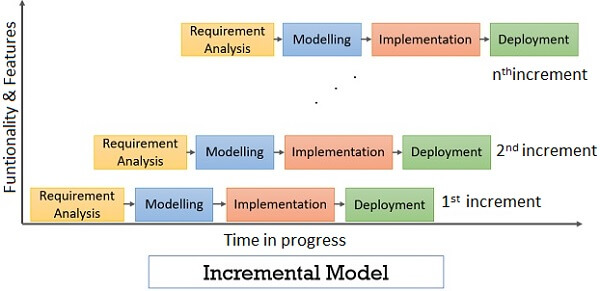
\includegraphics[width=\textwidth]{../../Immagini/ModelloIncrementale}
    \caption{Modello incrementale, Fonte: \href{https://binaryterms.com/incremental-development-model.html}{binaryterms.com}}
    \label{fig:modello_incrementale}
\end{figure}

In un modello di sviluppo incrementale, sulla base dei requisiti fondamentali e desiderabili trovati durante l'attività di analisi, vengono individuati degli incrementi da eseguire. Ogni incremento rappresenta un sottoinsieme delle funzionalità del prodotto finale. I requisiti sono da sviluppare seguendo una priorità (dalla più alta alla più bassa) quindi il rilascio del prodotto non viene mai eseguito in un unico blocco, ma incrementalmente.\\
Una volta che gli incrementi sono stati identificati, vengono definiti nel dettaglio i requisiti che devono essere soddisfatti col primo incremento dando il via alla fase di sviluppo dell’incremento stesso.  Durante l’attività di Sviluppo è lecito aggiungere ulteriori requisiti che devono essere soddisfatti dagli incrementi successivi, durante i periodi di \textit{Progettazione di Dettaglio, Codifica, Collaudo} e \textit{Validazione}; non si possono invece andare a modificare i requisiti decisi durante i periodi di \textit{\AdR} e \textit{Progettazione Architetturale}. In questo modo al termine di ogni incremento il prodotto software avrà dei miglioramenti o delle funzionalità aggiuntive dalle quali si può ricavare il grado di \glo{efficacia}. Ogni incremento quindi ridurrà il rischio di fallimento e produrrà valore aggiunto.\\
I vantaggi principali del modello di sviluppo incrementale sono:
\begin{itemize}
    \item Ogni incremento permette di avere un riscontro da parte del \glo{proponente};
    \item I requisiti a maggior priorità saranno i primi ad essere svilupatti e saranno anche più volte verificati nel corso dello sviluppo;
    \item Al termine di ogni incremento verrà effettuata la verifica dello stesso quindi eventuali errori saranno limitati al singolo incremento;
    \item Dall'incremento corrente è possibile trarre indicazioni su come effettuare il successivo;
    \item Grazie ai rilasci continui è possibile avere anticipatamente un prototipo da poter mostrare al proponente.
\end{itemize}

Come richiesto da \Proponente\ la parte di \glo{implementation} riguardante lo sviluppo in figura \S\ref{fig:modello_incrementale} è suddivisa in 4 ulteriori attività:
\begin{itemize}
    \item Sviluppo \glo{Locale};
    \item \glo{Test};
    \item \glo{Staging};
    \item \glo{Produzione} , equivale all'attività di \glo{deployment} presente in figura \S\ref{fig:modello_incrementale}.
\end{itemize}

\newpage

\section{Pianificazione}
\label{pianificazione}
Considerate le scadenze scelte in sottosezione \S\ref{sub:scadenze_fissate} ed il modello di sviluppo scelto presente nella sezione \S\ref{modello_di_sviluppo}, {\Gruppo} ha suddiviso il progetto in 5 periodi:
\begin{itemize}
    \item \textbf{Analisi};
    \item \textbf{Consolidamento Requisiti};
    \item \textbf{Progettazione Architetturale};
    \item \textbf{Progettazione di Dettaglio e Codifica};
    \item \textbf{Validazione e Collaudo};
\end{itemize}
 Ogni periodo è caratterizzato da \glo{precondizioni}, \glo{postcondizioni} ed è diviso in diversi \glo{stadi temporali}. Ognuno di questi cinque periodi sarà formato da \glo{attività} mostrate nei corrispettivi \textit{diagrammi di \glo{Gantt}}.Ogni attività si ramifica in sotto-attività per mostrarne l'esecuzione ad alto livello.

\subsection{Analisi}
\label{analisi}
\textbf{Durata:} dal 2020\_11\_06 al 2021\_01\_11\\
Durante questo periodo si forma il gruppo che si prepara alla \glo{\textbf{RR}}, studiando i \glo{capitolati} proposti e svolgendo un'analisi preliminare dei requisiti e la pianificazione globale del lavoro da svolgere. 
Le precondizioni sono:
\begin{itemize}
    \item Formazione del gruppo;
    \item Presentazione dei \glo{capitolati}.
\end{itemize}
Le postcondizioni sono:
\begin{itemize}
    \item Scelta del nome e del logo del gruppo;
    \item Creazione della mail e di un \glo{repository} \glo{GitHub};
    \item Scelta del capitolato;
    \item Redazione dei documenti quali: {\SdF}, {\NdP}, {\PdP}, {\Glossario}, \textit{Lettera di presentazione}, {\PdQ}, {\AdR} ed i verbali;
    \item Verifica e approvazione di quanto redatto.
\end{itemize}
Questa periodo è composto da sette attività che corrispondono ai documenti prodotti:
\begin{itemize}
    \item \textbf{Studio di fattibilità:} Vengono analizzati i vari capitolati per evidenziarne gli aspetti negativi e positivi. Dopo un periodo di studio e confronto {\Gruppo} dà la preferenza in quello più adatto. L'attività è bloccante per l'{\AdR};
    \item \textbf{Norme di progetto:} Vengono definite tutte le regole che il gruppo {\Gruppo} dovrà seguire per la stesura dei documenti e per lo sviluppo del progetto;
    \item \textbf{Glossario:} Contiene tutti i termini che possono risultare ambigui durante lo svolgimento del progetto; di essi viene fornita una definizione sintetica ed esaustiva;
    \item \textbf{Lettera di presentazione:} Documento in cui il gruppo {\Gruppo} si candida al capitolato scelto come fornitore del prodotto software richiesto;
    \item \textbf{Piano di progetto:} Nel presente documento sono descritte le attività, i rischi del progetto e viene calcolato il preventivo per la realizzazione di progetto. Presenta poi la suddivisione del lavoro tra i membri del gruppo {\Gruppo} e il calcolo del preventivo;
    \item \textbf{Analisi dei requisiti:} Vengono studiati e analizzati nel dettaglio i requisiti del capitolato scelto nello {\SdF};
    \item \textbf{Piano di qualifica:} Si individuano metodi e procedure per garantire la \glo{qualità} del prodotto.
\end{itemize}
La pianificazione di questo periodo è stata organizzata nel modo seguente:
\begin{enumerate}
\item \textbf{2020\_11\_06 - 2020\_12\_03}:
Inizio della stesura delle {\NdP} per avere delle regole condivise dal gruppo per svolgere il lavoro. Durante la stesura di queste, il gruppo si confronta riguardo ai vari capitolati esponendo le preferenze personali di ciascun componente del gruppo. Viene analizzato ogni capitolato focalizzando l'attenzione principalmente verso i loro aspetti positivi e negativi e dei possibili rischi che si possono incontrare per ognuno. Dopo i confronti iniziali si è potuto iniziare uno studio sulla fattibilità generico per tutti i capitolati per poi approfondirlo per i capitolati che suscitavano più interesse al gruppo e iniziare a stilare il {\Glossario} per la registrazione dei termini, usati nei documenti, che potrebbero creare ambiguità. Durante questo periodo sono state prese decisioni tecniche e organizzative come: nome del gruppo, logo, indirizzo mail, creazione \glo{repository} e i vari mezzi di comunicazione. Vengono trascritti i verbali interni relativi alle riunioni del gruppo durante questo arco di tempo;
\item \textbf{2020\_12\_04 - 2020\_12\_21}:
Inizio della stesura del {\PdP}, contenente la pianificazione del lavoro da svolgere e la suddivisione dei ruoli tra i membri del gruppo. Stesa una prima bozza della \textit{Lettera di presentazione}, il cui completamento sarà fatto dopo la conclusione del {\PdP} con l'aggiunta del prospetto economico finale. Integrato il {\Glossario} quando necessario. In data 2020\_12\_22 il gruppo ha fissato una \glo{milestone} per il completamento dei documenti iniziati durante questo periodo, ad eccezione dell'ultima sezione del {\PdP} destinata al consuntivo finale del periodo successivo. Iniziano le attività di verifica incrementale per i documenti in corso di stesura. Stesi i verbali interni relativi agli incontri svolti;
\item \textbf{2020\_12\_22 - 2021\_01\_07}:
Inizio della stesura dell'{\AdR} e del {\PdQ}, con l'esposizione dei criteri di valutazione della qualità scelti dal gruppo e le rispettive metriche di calcolo. Continuano le attività di verifica incrementale per i documenti in corso di stesura;
\item \textbf{2021\_01\_08 - 2021\_01\_11}
Il gruppo svolge le ultime attività di verifica sugli ultimi documenti, completa il {\Glossario} e uniforma tutti i prodotti alle regole stabilite nelle {\NdP} se necessario.
\end{enumerate}
\subsubsection{Diagramma di Gantt: Analisi}
\begin{figure}[ht]
    \centering
    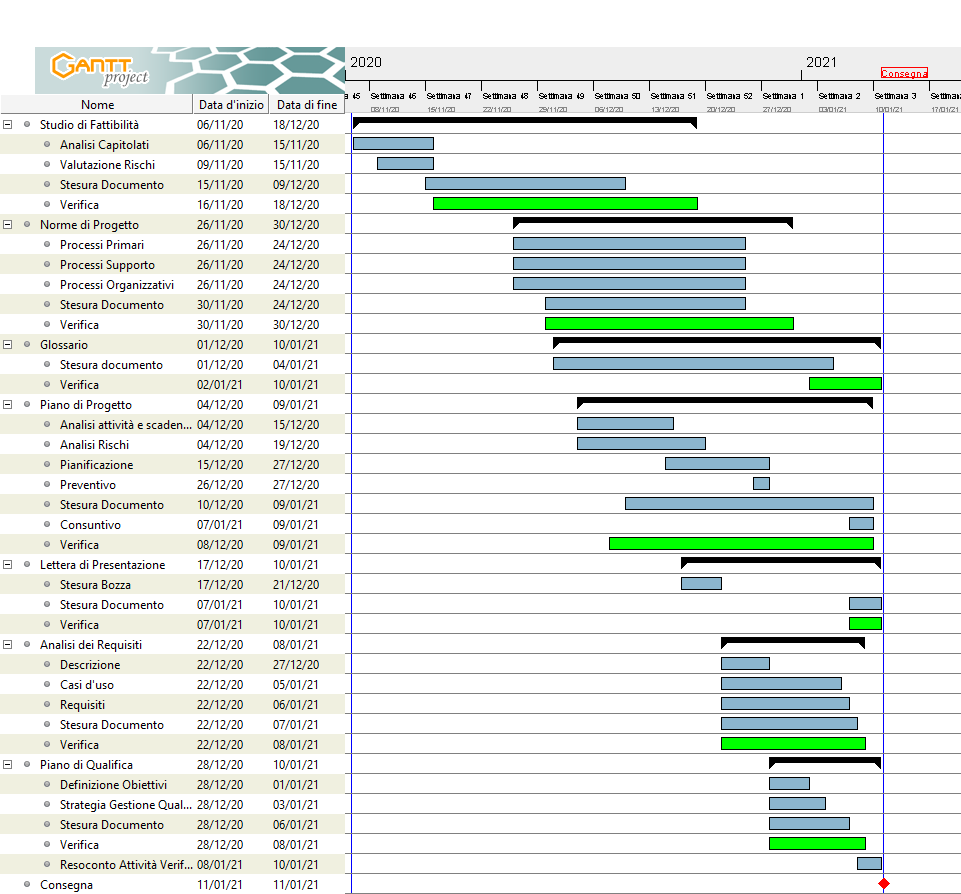
\includegraphics[width=\textwidth]{Immagini/GanttAnalisi}
    \caption{Diagramma di Gantt dell'attività di analisi}
\end{figure}
\newpage
\subsection{Consolidamento Requisiti}
\label{consolidamento_requisiti}
\textbf{Durata:} dal 2020-01-11 al 2020-01-18 \\
In questo periodo il gruppo si prepara alla propria presentazione in vista della \textit{Revisione dei Requisiti}.
I componenti si dividono gli argomenti da esporre e descrivono il lavoro svolto durante l'analisi attraverso delle diapositive.
I membri del team si occupano di approfondire individualmente la propria conoscenza delle tecnologie che verranno utilizzate successivamente.

Le precondizioni sono:
\begin{itemize}
    \item Le postcondizioni del periodo precedente sono state soddisfatte;
    \item Consegna dei documenti richiesti al proponente.
\end{itemize}

Le postcondizioni sono:
\begin{itemize}
    \item Ultimata preparazione della presentazione da esporre in sede di revisione;
    \item Ogni componente ha studiato le tecnologie necessarie;
\end{itemize}
Le attività che vengono svolte sono:
\begin{itemize}
    \item Miglioramento dei documenti e verifica;
    \item Preparazione alla presentazione per la \textit{Revisione dei Requisiti};
    \item Ogni componente dovrà svolgere dello studio autonomo per approfondire le tecnologie necessarie nei periodi successivi.  
\end{itemize}

\newpage
\subsubsection{Diagramma di Gantt: Consolidamento Requisiti}
\begin{figure}[ht]
    \centering
    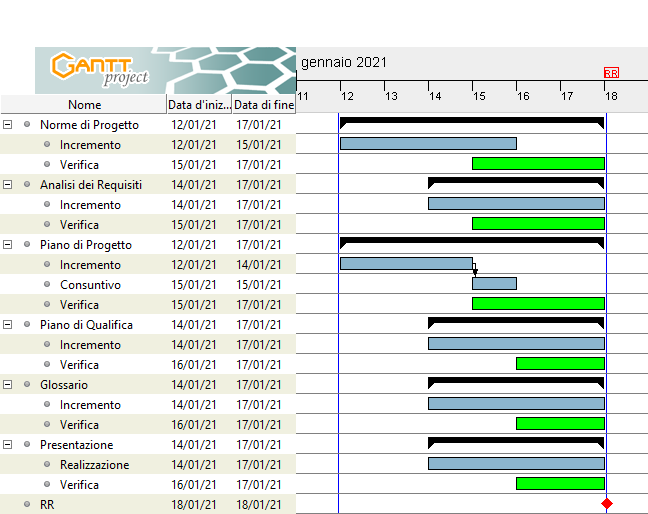
\includegraphics[width=\textwidth]{../../Immagini/GanttConsolidamentoRequisiti}
    \caption{Diagramma di Gantt dell'avvitià di Consolidamento dei Requisiti}
\end{figure}

\newpage
\subsection{Progettazione Architetturale}

\textbf{Periodo:} dal 2020-01-18 al 2020-03-08
\\La fase inizia appena conclusa la precedente e termina con la Revisione di Progettazione.
\\Le precondizioni sono:

\begin{itemize}
    \item Le postcondizioni della fase precedente sono state soddisfatte;
    \item La candidatura del gruppo al progetto \NomeProgetto è stata accolta.
\end{itemize}
    Le postcondizioni sono:
\begin{itemize}
    \item Aggiornamento e correzione dei documenti già prodotti;
    \item Produzione del Proof of Concept;
    \item Completamento della progettazione ad alto livello del software;
    \item Consegna dei documenti richiesti in entrata allaRevisione di Progettazione;
    \item Ultimata preparazione della presentazione da esporre in sede di revisione.
\end{itemize}

\subsubsection{Attività}

\subsubsection{Periodi}

\subsubsection{Diagramma di Gantt: Progettazione Architetturale}

\newpage
\subsection{Progettazione di dettaglio e codifica}
\label{progettazione_di_dettaglio}
\textbf{Durata:} dal 2021\_03\_09 al 2021\_04\_02 \\
Il periodo inizia appena concluso il precedente e termina con la \glo{\textbf{RQ}}.
Le precondizioni sono:
\begin{itemize}
    \item Le postcondizioni del periodo precedente sono state soddisfatte.
\end{itemize}
Le postcondizioni sono:
\begin{itemize}
    \item Aggiornamento e correzione dei documenti già prodotti;
    \item Realizzazione dei diagrammi delle classi e delle attività;
    \item Completamento codifica e relativa verifica;
    \item Redazione \textbf{manuale utente} e \textbf{manuale sviluppatore};
    \item Consegna dei documenti richiesti in entrata alla \textbf{RQ};
    \item Ultimata preparazione della presentazione da esporre in sede di revisione.
\end{itemize}
È composto da nuovi incrementi e nuove attività:
\begin{itemize}
    \item \textbf{Incremento e verifica dei documenti (dal 2021\_03\_09 al 2021\_03\_26):} i documenti già prodotti vengono migliorati e aggiornati se necessario ({\NdP}, {\PdP}, {\Glossario}, {\PdQ}, {\AdR});
    \item \textbf{Incremento e verifica delle attività (dal 2021\_03\_09 al 2021\_03\_17)}: viene migliorata l'attività di \glo{TB}, ampliando lo studio delle tecnologie mancanti e progettando ad alto livello come realizzare il prodotto finale;
    \item \textbf{Product Baseline (dal 2021\_03\_09 al 2021\_03\_17):} segue la Technology Baseline e vengono discussi:
        \begin{itemize}
            \item \textbf{Design pattern}: vengono individuati e discussi in modo da capire quali siano necessari e come riuscire a integrarli al meglio nel progetto;
            \item \textbf{Diagrammi classi}: dopo un'attenta riflessione sul codice vengono realizzati i diagrammi delle classi;
            \item \textbf{Diagrammi attività}: dopo un'attenta riflessione sul codice vengono realizzati i diagrammi delle attività. 
        \end{itemize} 
    \item \textbf{Specifica tecnica(dal 2021\_03\_18 al 2021\_03\_26):} viene realizzato un documento contenente tutte le caratteristiche del prodotto e le motivazioni che hanno portato alla loro scelta;
    \item \textbf{Codifica (dal 2021\_03\_18 al 2021\_04\_06):} viene scritto il codice con relativa verifica. Questa attività, dato il modello di sviluppo scelto, verrà suddivisa in 3 incrementi che verranno definiti dopo aver preparato il Proof of Concept così da avere una maggiore conoscenza sul lavoro effettivo da svolgere e poter progettare al meglio i vari incrementi;
    \item \textbf{Manuale utente e manutentore(dal 2021\_03\_24 al 2021\_04\_06):} documenti redatti rispettivamente per indicare le istruzioni d'uso specifiche per l'utente e per supportare eventuali sviluppatori attraverso la descrizione dell'architettura del sistema.
\end{itemize}
\subsubsection{Incrementi del periodo}\label{IncrementiPDettaglio}
\begin{table}[H]
	\begin{center}
		\begin{tabular}{ |C{3cm} C{6cm} C{7cm}| }
			\rowcolor{darkblue} 
			\textcolor{white}{\textbf{Incremento}} & \textcolor{white}{\textbf{Obiettivi}} & \textcolor{white}{\textbf{Requisiti}} \\ \hline
			I dal 2021\_03\_09 al 2021\_03\_17& Miglioramento della documentazione già prodotta, ampliamento dello studio delle tecnologie, studio di \glo{design pattern}, diagrammi delle classi e delle attività.  & - \\ \hline
			II dal 2021\_03\_18 al 2021\_03\_26 	& Correzione dei documenti post \glo{RP}, redazione dell'allegato tecnico, inizio sviluppo del codice e redazione manuali. &  
			RFO1\_1 - RFO6\_1.1.5, RFO7\_2 \newline
			RFO8\_3, RFO10\_4, RFO11\_5 \newline
			RFO59, RFO60 \newline
			RFO61\_23 - RFO62\_23.4, RFO67\_25 \newline
			RF069, RFO70\_26 - RFO77\_26.7 \newline
			RFO78, RFO79, RFO12\_6, \newline 
			RFO13\_ 7 - RFO15\_ 7.3, RFO17 \newline RFO18, RFO19, RFO20\_8\newline RFO21\_9, RFO22\_10, RFO23\_11 \newline RFO24, RFO27, RFO28 \newline RFO29\_12, RFO68, RFO80 \newline RFO81, RFO82, RFO80 \\ \hline
			III dal 2021\_03\_27 al 2021\_04\_01 	& Continuazione nello sviluppo del codice e nella redazione manuali. & RFO81\_27 - RFO88\_27.7 \newline
			RFO89, RFO90\_28 - RFO97\_28.7 \newline
			RFO98\_29, RFO99\_30, RFO100\_31 \newline
			RFO101\_32, RFO102\_33 \newline
			RFO103\_34 - RFO107\_34.4, RFO108 \newline
			RFO109\_35 - RFO110\_35.1\newline
			RFO111\_36 - RFO112\_36.1, RFO113\_37 \newline RFO114\_38, RFO115, RFO26 \newline RFO30\_13, RFO31, RFO32\_14 \newline RFO33\_14, RFO34\_15, RFO35\_16\newline  RFO36, RFO37, RFO41\_17.2 \\ \hline
			III dal 2021\_04\_01 al 2021\_04\_06 	& 
			Conclusione della redazione del codice e dei manuali. & RFO24, RFO41\_17, RFO39\_17.1\newline RFO40,
			RFO41\_17 - RFO45\_17.1.4\newline
			RFO46\_18 - RFO50\_18.4, RFO51\_19 \newline
			RFO52, RFO53\_20, RFO54\_20 \newline
			RFO55\_21, RFO56\_22 - RFO58\_22.2 \newline
			RFO79, RFO116\_39, RFO117\_39 \newline RFO118\_40, RFO119, RFO120\_41 \newline
			RFO121\_42, RFO122\_43 - RFO126\_43.2.2 \\ \hline
		\end{tabular}
		\caption{Tracciamento incrementi-obiettivi}
	\end{center}
\end{table}

\newpage
\subsubsection{Diagramma di Gantt: Progettazione di dettaglio e codifica} \label{GanttPDettaglio}
\begin{figure}[ht]
    \centering
    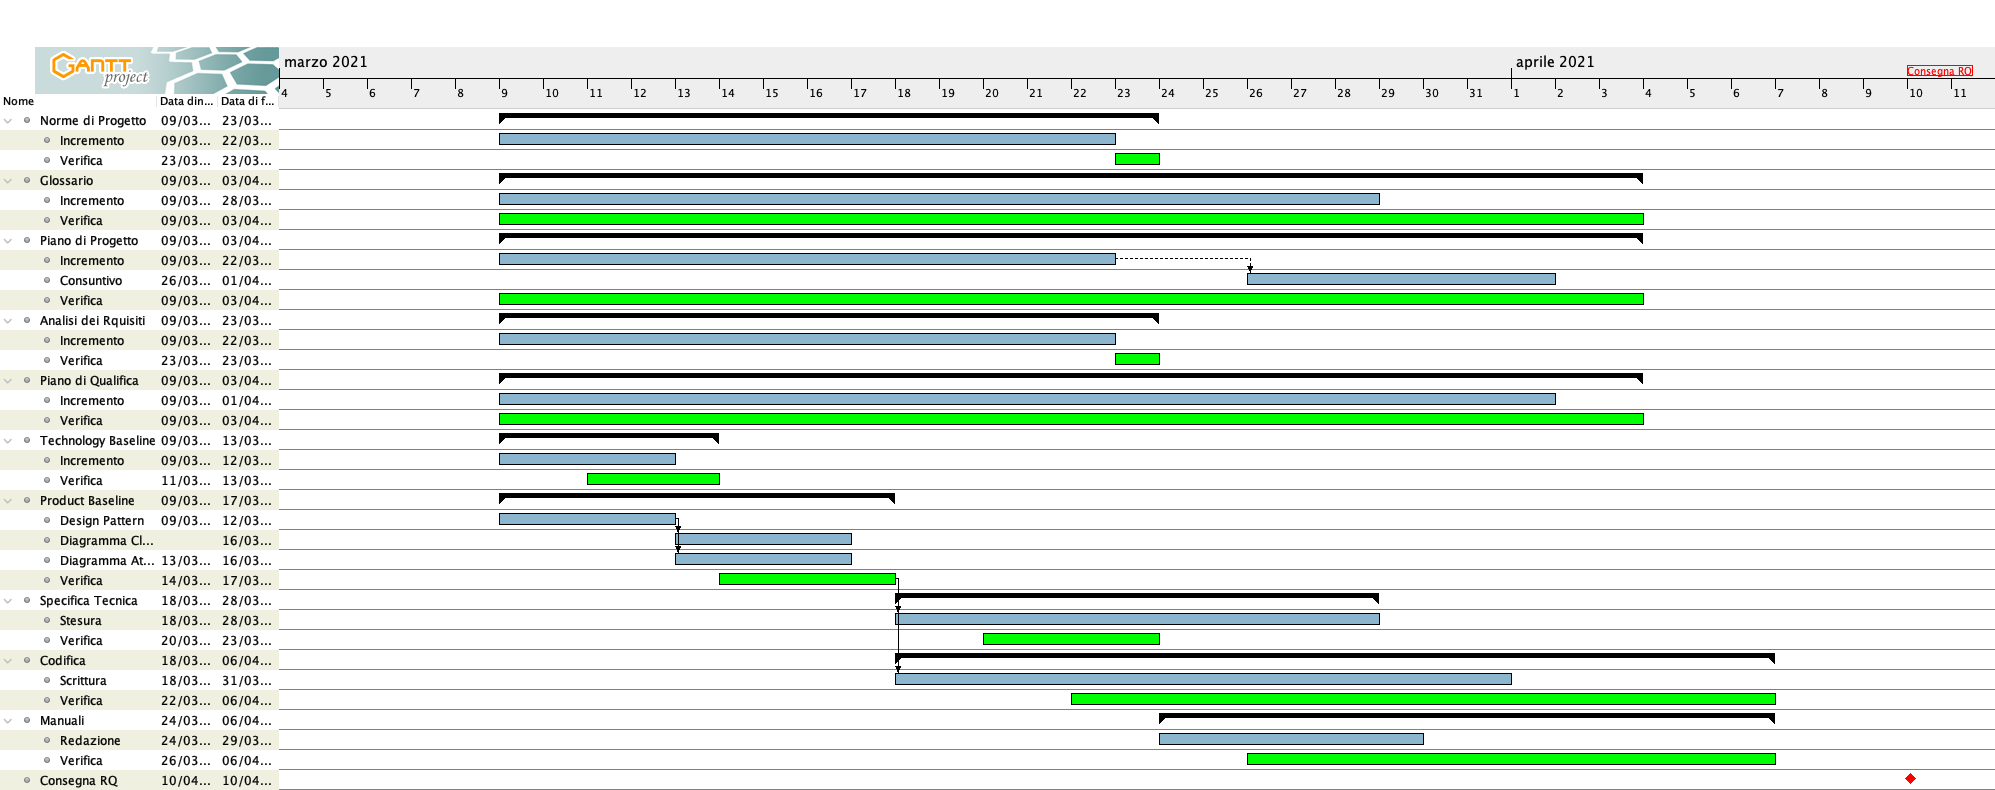
\includegraphics[width=\textwidth]{Immagini/GanttProgettazioneDiDettaglioECodifica}
    \caption{Diagramma di Gantt dell'attività di progettazione di dettaglio e codifica}
\end{figure}
\newpage
\subsection{Validazione e collaudo}
\label{validazione_e_collaudo}
\textbf{Durata:} dal 2021\_05\_01 al 2021\_05\_19\\
Il periodo di validazione e collaudo inizia appena concluso il precedente e termina con la \glo{\textbf{RA}}.
Le precondizioni sono:
\begin{itemize}
    \item Le postcondizioni del periodo precedente sono state soddisfatte.
\end{itemize}
Le postcondizioni sono:
\begin{itemize}
    \item Aggiornamento e correzione documenti già prodotti;
    \item Esecuzione dei vari test;
    \item Completamento del prodotto in base a quanto discusso durante la \textbf{RQ};
    \item Consegna dei documenti richiesti in entrata alla \textbf{RA};
    \item Ultimata preparazione della presentazione da esporre in sede di revisione.
\end{itemize}
È composto da nove incrementi e una nuova attività:
\begin{itemize}
    \item \textbf{Incremento e verifica dei documenti}: alcuni dei documenti già prodotti vengono migliorati e aggiornati ({\NdP}, {\PdP}, {\Glossario}, {\PdQ}, \textit{Specifica tecnica}, \textit{Manuale utente}); 
    \item \textbf{Incremento e verifica delle attività}: se necessario vengono migliorate le attività di \textbf{Technology Baseline} per quanto riguarda la progettazione ad alto livello, in particolare la \textbf{Product Baseline} riguardo all'aggiunta di design pattern o di diagrammi di classi o di attività; la parte di codifica, in caso non siano stati riscontrati rallentamenti o ritardi nel progetto, potrebbe comprendere l'implementazione di uno o più casi d'uso opzionali;
    \item \textbf{Validazione e collaudo}: realizzazione degli ultimi test, con successivi controlli finali per garantire un buon livello di qualità e correttezza.
\end{itemize}
\newpage
\subsubsection{Ripianificazione attuata relativa al periodo} \label{RipianificazioneValidazione}
A seguito dei ritardi accumulati nei periodi precedenti si prevede di consegnare il prodotto verso metà maggio rispettando comunque il preventivo concordato precedentemente e il livello di qualità che il gruppo intende assicurare. Di seguito si riporta il nuovo diagramma di Gantt considerando la nuova data di consegna del prodotto.
\subsubsection{Diagramma di Gantt: Validazione e collaudo}\label{GanttValidazione}
\begin{figure}[ht]
    \centering
    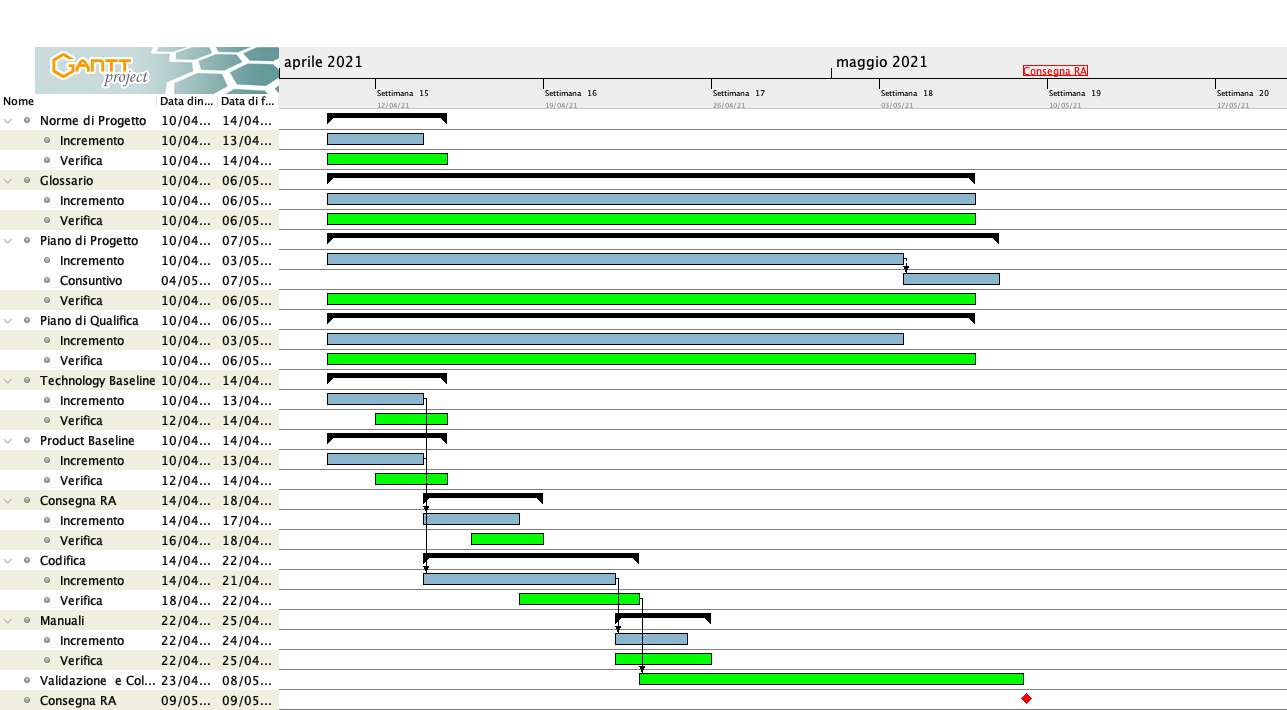
\includegraphics[width=\textwidth]{Immagini/GanttValidazioneECollaudo}
    \caption{Diagramma di Gantt dell'attività di validazione e collaudo}
\end{figure}
\newpage

\newpage

\section{Preventivo}
\label{preventivo}
Per ogni periodo individuato nella sezione \S\ref{pianificazione} relativa alla pianificazione, si espone un prospetto orario dove sono raccolte le ore che ciascun membro deve svolgere per ruolo.\\Viene successivamente mostrato un prospetto economico che riassume i costi sostenuti per ciascun ruolo.\\
Per agevolare la lettura delle tabelle, se un membro del gruppo non ha ricoperto un certo ruolo verrà inserito il simbolo \textbf{-} per indicarne l'assenza.\\Si è poi pensato di utilizzare le seguenti sigle per identificare i ruoli:
\begin{itemize}
\item \textbf{Re:} \textit{\Responsabile};
\item \textbf{Am:} \textit{\Amministratore};
\item \textbf{An:} \textit{Analista};
\item \textbf{Pt:} \textit{Progettista};
\item \textbf{Pr:} \textit{Programmatore};
\item \textbf{Ve:} \textit{Verificatore}.
\end{itemize}
\newpage

\subsection{Periodo di Analisi}
\subsubsection{Prospetto orario}
In questo periodo, ogni componente del gruppo rivestirà i seguenti ruoli:
\begin{table}[H]
	\begin{center}
		\begin{tabular}{ |c c c c c c c c|}
		\rowcolor{darkblue} 
		\textcolor{white}{\textbf{Nominativo}} & \textcolor{white}{\textbf{Re}} & \textcolor{white}{\textbf{Am}} & \textcolor{white}{\textbf{An}} & \textcolor{white}{\textbf{Pt}} & \textcolor{white}{\textbf{Pr}} & \textcolor{white}{\textbf{Ve}} & \textcolor{white}{\textbf{Ore Complessive}} \\ \hline
		\BL 	& - 	& 6 	& 16 	& - 	& - 	& 8 	& 30 \\ \hline
		\FF 	& - 	& 5 	& 15 	& - 	& - 	& 10 	& 30 \\ \hline
		\MM		& 15	& - 	& 10 	& - 	& - 	& 5 	& 30 \\ \hline
		\PC		& 5 	& 4 	& 10 	& - 	& - 	& 11	& 30 \\ \hline
		\TG 	& - 	& 15	& 10 	& - 	& - 	& 5 	& 30 \\ \hline
		\TL 	& 4 	& 5 	& 16 	& - 	& - 	& 5 	& 30 \\ \hline
		\VD 	& - 	& -  	& 12 	& - 	& - 	& 18 	& 30 \\ \hline
		\textbf{Ore totali} & \textbf{24} & \textbf{35} & \textbf{89} & \textbf{-} & \textbf{-} & \textbf{62} & \textbf{210} \\ \hline
		\end{tabular}
	\caption{Distribuzione delle ore nel periodo di Analisi}
	\end{center}
\end{table}
I dati ottenuti vengono riassunti nel seguente istogramma:
\begin{figure}[H]
    \centering
    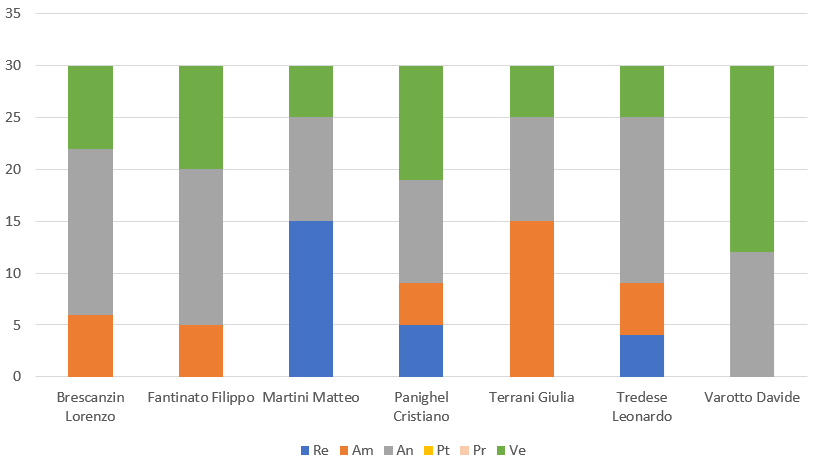
\includegraphics[scale = 0.70]{Immagini/AnalisiIsto.png}
    \caption{Istogramma della ripartizione delle ore per ruolo in Analisi}
    \label{fig:istogramma ripartizione ore, periodo di Analisi}
\end{figure}
\newpage
\subsubsection{Prospetto economico}
Il costo per ogni ruolo è il seguente:
\begin{table}[H]
	\begin{center}
		\begin{tabular}{ |c c c| }
		\rowcolor{darkblue} 
		\textcolor{white}{\textbf{Ruolo}} & \textcolor{white}{\textbf{Ore}} & \textcolor{white}{\textbf{Costo}} \\ \hline
		\textit{\Responsabile} 		& 24 	& 720€ \\ \hline
		\textit{\Amministratore} 	& 35 	& 700€ \\ \hline
		\textit{Analista} 			& 89 	& 2225€ \\ \hline
		\textit{Progettista} 		& - 	& - \\ \hline
		\textit{Programmatore}  	& - 	& - \\ \hline
		\textit{Verificatore} 		& 62 	& 930€ \\ \hline
		\textbf{Totale} 			& \textbf{210} & \textbf{4575€} \\ \hline
		\end{tabular}
	\caption{ Prospetto dei costi per ruoli nel periodo di Analisi}
	\end{center}
\end{table}
Il seguente grafico a torta riassume i dati ottenuti:
\begin{figure}[H]
    \centering
    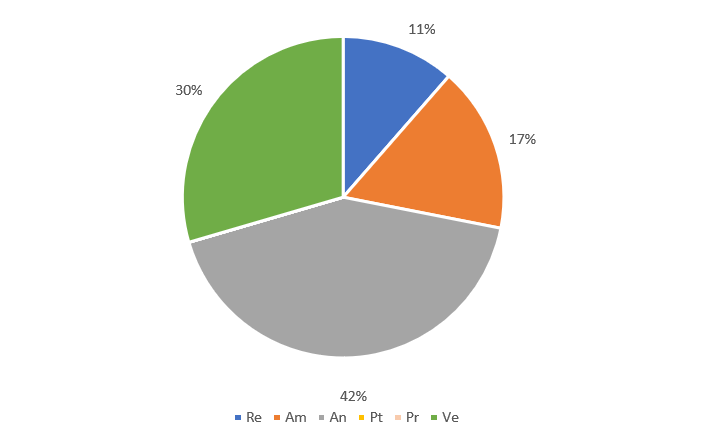
\includegraphics[scale = 0.75]{Immagini/AnalisiTorta.png}
    \caption{Areogramma ripartizione ore, periodo di Analisi}
    \label{fig:Areogramma ripartizione ore, periodo di Analisi}
\end{figure}
\newpage

\subsection{Periodo di Consolidamento dei Requisiti}
\subsubsection{Prospetto orario}
Durante il periodo di Consolidamento dei Requisiti viene effettuata la seguente distribuzione oraria:
\begin{table}[H]
	\begin{center}
		\begin{tabular}{ |c c c c c c c c| }
		\rowcolor{darkblue} 
		\textcolor{white}{\textbf{Nominativo}} & \textcolor{white}{\textbf{Re}} & \textcolor{white}{\textbf{Am}} & \textcolor{white}{\textbf{An}} & \textcolor{white}{\textbf{Pt}} & \textcolor{white}{\textbf{Pr}} & \textcolor{white}{\textbf{Ve}} & \textcolor{white}{\textbf{Ore Complessive}} \\ \hline
		\BL 	& - 	& 3  	& - 	& 3 	& - 	& - 	& 6 \\ \hline
		\FF 	& - 	& 3  	& 3 	& - 	& - 	& -  	& 6 \\ \hline
		\MM 	& -  	& -  	& 2 	& - 	& - 	& 4  	& 6 \\ \hline
		\PC 	& - 	& -  	& 4 	& 2 	& - 	& - 	& 6 \\ \hline
		\TG 	& 2  	& - 	& 4 	& - 	& - 	& - 	& 6 \\ \hline
		\TL 	& 3  	& - 	& - 	& - 	& - 	& 3 	& 6 \\ \hline
		\VD 	& -  	& -  	& 4 	& 2 	& - 	& -  	& 6 \\ \hline
		\textbf{Ore totali} & \textbf{5} & \textbf{6} & \textbf{17} & \textbf{7} & \textbf{-} & \textbf{7} & \textbf{42} \\ \hline
		\end{tabular}
	\caption{Distribuzione delle ore nel periodo di Consolidamento dei Requisiti}
	\end{center}
\end{table}
I dati ottenuti vengono riassunti nel seguente istogramma:
\begin{figure}[H]
    \centering
    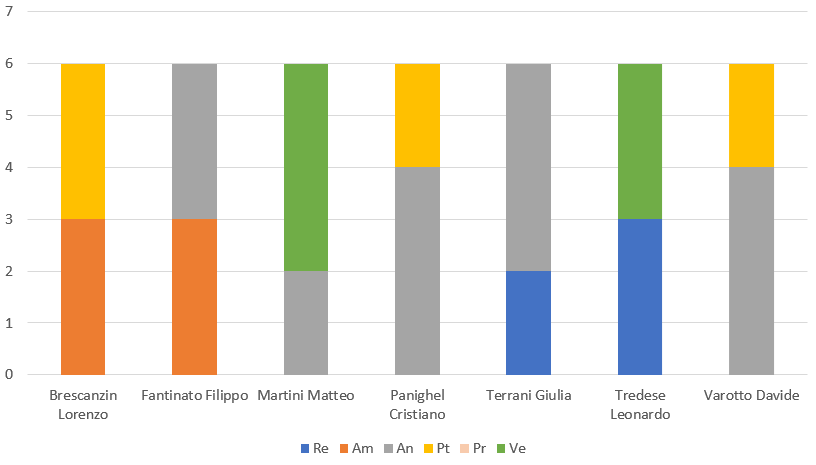
\includegraphics[scale = 0.70]{Immagini/ConsolidamentoIsto.png}
    \caption{Istogramma della ripartizione delle ore per ruolo in Consolidamento dei Requisiti}
    \label{fig:istogramma ripartizione ore, periodo di Consolidamento dei Requisiti}
\end{figure}
\newpage
\subsubsection{Prospetto economico}
Il costo per ogni ruolo è il seguente:
\begin{table}[H]
	\begin{center}
		\begin{tabular}{ |c c c|}
		\rowcolor{darkblue} 
		\textcolor{white}{\textbf{Ruolo}} & \textcolor{white}{\textbf{Ore}} & \textcolor{white}{\textbf{Costo}} \\ \hline
		\textit{\Responsabile} 		& 5 	& 150€ \\ \hline
		\textit{\Amministratore} 	& 6 	& 120€ \\ \hline
		\textit{Analista} 			& 17 	& 425€ \\ \hline
		\textit{Progettista} 		& 7 	& 154€ \\ \hline
		\textit{Programmatore}  	& - 	& - \\ \hline
		\textit{Verificatore} 		& 7 	& 105€ \\ \hline
		\textbf{Totale} 			& \textbf{42} & \textbf{954€} \\ \hline
		\end{tabular}
	\caption{ Prospetto dei costi per ruoli nel periodo di Consolidamento dei Requisiti}
	\end{center}
\end{table}
Il seguente grafico a torta riassume i dati ottenuti:
\begin{figure}[H]
    \centering
    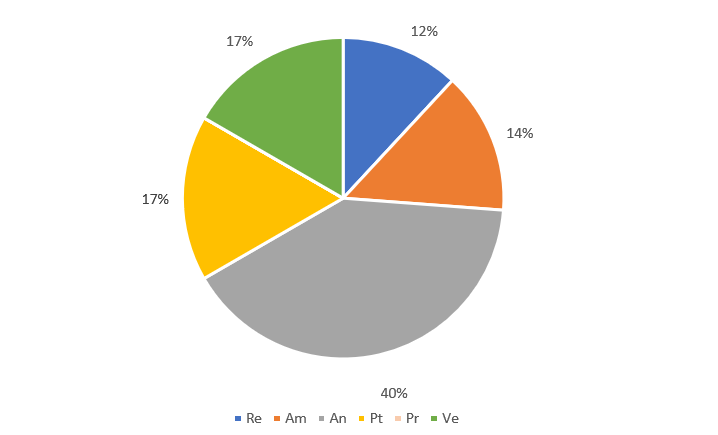
\includegraphics[scale = 0.75]{Immagini/ConsolidamentoTorta.png}
    \caption{Areogramma della ripartizione di ore per ruolo in Consolidamento dei Requisiti}
    \label{fig:Areogramma ripartizione ore, periodo di Consolidamento dei Requisiti}
\end{figure}
\newpage

\subsection{Periodo di Progettazione Architetturale}
\subsubsection{Prospetto orario}
In questo periodo la distribuzione oraria è la seguente:
\begin{table}[H]
	\begin{center}
		\begin{tabular}{ |c c c c c c c c| }
		\rowcolor{darkblue} 
		\textcolor{white}{\textbf{Nominativo}} & \textcolor{white}{\textbf{Re}} & \textcolor{white}{\textbf{Am}} & \textcolor{white}{\textbf{An}} & \textcolor{white}{\textbf{Pt}} & \textcolor{white}{\textbf{Pr}} & \textcolor{white}{\textbf{Ve}} & \textcolor{white}{\textbf{Ore Complessive}} \\ \hline
		\BL 	& -  	& -  	& 8 	& 12 	& 3 	& 7 	& 30 \\ \hline
		\FF 	& 3  	& -  	& - 	& 16 	& 5 	& 6  	& 30 \\ \hline
		\MM 	& -  	& 3  	& 10 	& 8 	& 5 	& 4  	& 30 \\ \hline
		\PC 	& - 	& -  	& 10 	& - 	& 4 	& 16 	& 30 \\ \hline
		\TG 	& -  	& 3 	& 10 	& 13 	& - 	& 4 	& 30 \\ \hline
		\TL 	& 5  	& 6 	& - 	& - 	& 4 	& 15 	& 30 \\ \hline
		\VD 	& 10  	& 8  	& - 	& 12 	& - 	& -  	& 30 \\ \hline
		\textbf{Ore totali} & \textbf{18} & \textbf{20} & \textbf{38} & \textbf{61} & \textbf{21} & \textbf{52} & \textbf{210} \\ \hline
		\end{tabular}
	\caption{Distribuzione delle ore nel periodo di Progettazione Architetturale}
	\end{center}
\end{table}
I dati ottenuti vengono riassunti nel seguente istogramma:
\begin{figure}[H]
    \centering
    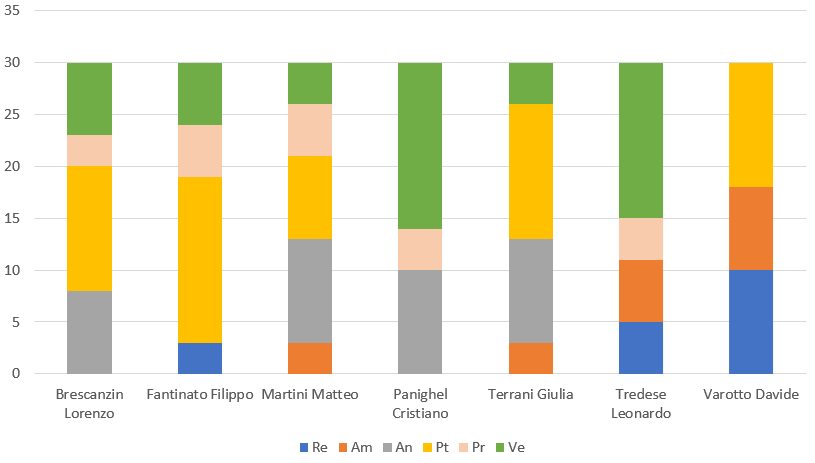
\includegraphics[scale = 0.70]{Immagini/ArchitetturaIsto.png}
    \caption{Istogramma della ripartizione delle ore per ruolo in Progettazione Architetturale}
    \label{fig:istogramma ripartizione ore, periodo di Progettazione Architetturale}
\end{figure}
\newpage
\subsubsection{Prospetto economico}
Il costo per ogni ruolo è il seguente:
\begin{table}[H]
	\begin{center}
		\begin{tabular}{ |c c c| }
		\rowcolor{darkblue} 
		\textcolor{white}{\textbf{Ruolo}} & \textcolor{white}{\textbf{Ore}} & \textcolor{white}{\textbf{Costo}} \\ \hline
		\textit{\Responsabile} 		& 18 & 540€ \\ \hline
		\textit{\Amministratore} 	& 20 & 400€ \\ \hline
		\textit{Analista} 			& 38 & 950€ \\ \hline
		\textit{Progettista} 		& 61 & 1342€\\ \hline
		\textit{Programmatore}  	& 21 & 315€ \\ \hline
		\textit{Verificatore} 		& 52 & 780€ \\ \hline
		\textbf{Totale} & \textbf{210} & \textbf{4327€} \\ \hline
		\end{tabular}
	\caption{ Prospetto dei costi per ruoli nel periodo di Progettazione Architetturale}
	\end{center}
\end{table}
Il seguente grafico a torta riassume i dati ottenuti:
\begin{figure}[H]
    \centering
    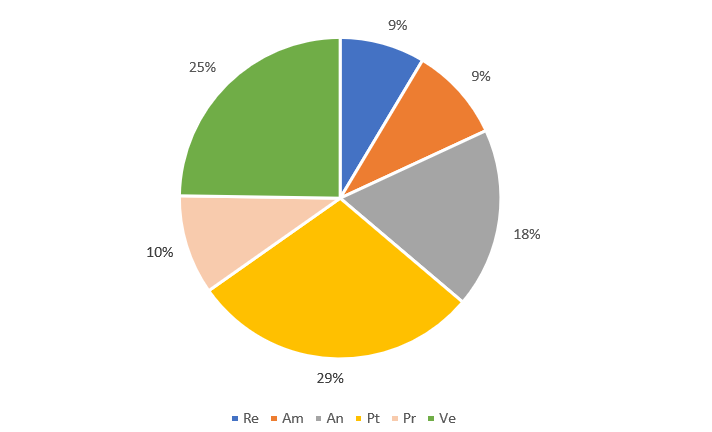
\includegraphics[scale = 0.75]{Immagini/ArchitetturaTorta.png}
    \caption{Areogramma della ripartizione di ore per ruolo in Progettazione Architetturale}
    \label{fig:Areogramma ripartizione ore, periodo di Progettazione Architetturale}
\end{figure}
\newpage

\subsection{Periodo di Progettazione di Dettaglio e Codifica}
\subsubsection{Prospetto orario}
In questo periodo la distribuzione oraria è la seguente:
\begin{table}[H]
	\begin{center}
		\begin{tabular}{ |c c c c c c c c| }
		\rowcolor{darkblue} 
		\textcolor{white}{\textbf{Nominativo}} & \textcolor{white}{\textbf{Re}} & \textcolor{white}{\textbf{Am}} & \textcolor{white}{\textbf{An}} & \textcolor{white}{\textbf{Pt}} & \textcolor{white}{\textbf{Pr}} & \textcolor{white}{\textbf{Ve}} & \textcolor{white}{\textbf{Ore Complessive}} \\ \hline
		\BL 	& 4  	& -  	& - 	& 15 	& 21 	& 10 	& 50 \\ \hline
		\FF 	& -  	& -  	& - 	& 30 	& 20 	& -  	& 50 \\ \hline
		\MM 	& -  	& 8  	& - 	& 15 	& 15 	& 12 	& 50 \\ \hline
		\PC 	& 5 	& 4  	& - 	& 11 	& 18 	& 12 	& 50 \\ \hline
		\TG 	& 5  	& 2		& - 	& 6 	& 20 	& 17 	& 50 \\ \hline
		\TL 	& -  	& - 	& - 	& 15 	& 20 	& 15 	& 50 \\ \hline
		\VD 	& 4  	& 4  	& - 	& 12 	& 20 	& 10 	& 50 \\ \hline
		\textbf{Ore totali} & \textbf{18} & \textbf{18} & \textbf{-} & \textbf{104} & \textbf{134} & \textbf{76} & \textbf{350} \\ \hline
		\end{tabular}
	\caption{Distribuzione delle ore nel periodo di Progettazione di Dettaglio e Codifica}
	\end{center}
\end{table}
I dati ottenuti vengono riassunti nel seguente istogramma:
\begin{figure}[H]
    \centering
    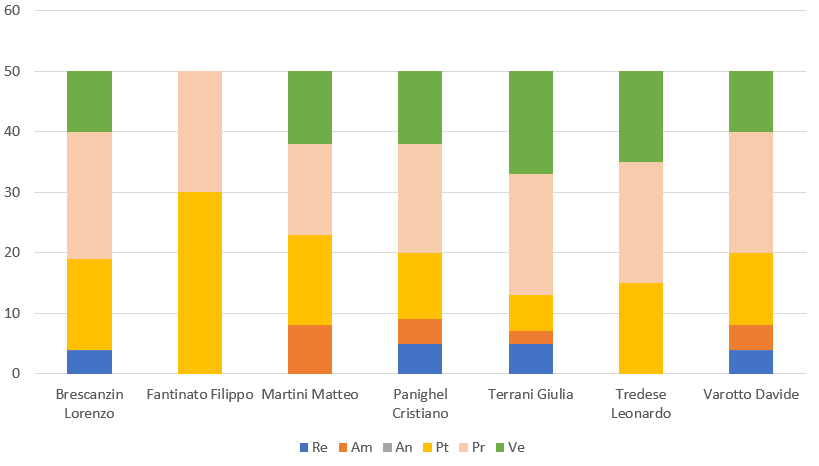
\includegraphics[scale = 0.70]{Immagini/DettaglioIsto.png}
    \caption{Istogramma della ripartizione delle ore per ruolo in Progettazione di Dettaglio e Codifica}
    \label{fig:istogramma ripartizione ore, periodo di Progettazione di Dettaglio e Codifica}
\end{figure}
\newpage
\subsubsection{Prospetto economico}
Il costo per ogni ruolo è il seguente:
\begin{table}[H]
	\begin{center}
		\begin{tabular}{ |c c c| }
		\rowcolor{darkblue} 
		\textcolor{white}{\textbf{Ruolo}} & \textcolor{white}{\textbf{Ore}} & \textcolor{white}{\textbf{Costo}} \\ \hline
		\textit{\Responsabile} 		& 18 	& 540€ \\ \hline
		\textit{\Amministratore} 	& 18 	& 360€ \\ \hline
		\textit{Analista} 			& - 	& - \\ \hline
		\textit{Progettista} 		& 104 	& 2288€ \\ \hline
		\textit{Programmatore}  	& 134 	& 2010€ \\ \hline
		\textit{Verificatore} 		& 76 	& 1140€ \\ \hline
		\textbf{Totale} & \textbf{350} & \textbf{6338€} \\ \hline
		\end{tabular}
	\caption{ Prospetto dei costi per ruoli nel periodo di Progettazione di Dettaglio e Codifica}
	\end{center}
\end{table}
Il seguente grafico a torta riassume i dati ottenuti:
\begin{figure}[H]
    \centering
    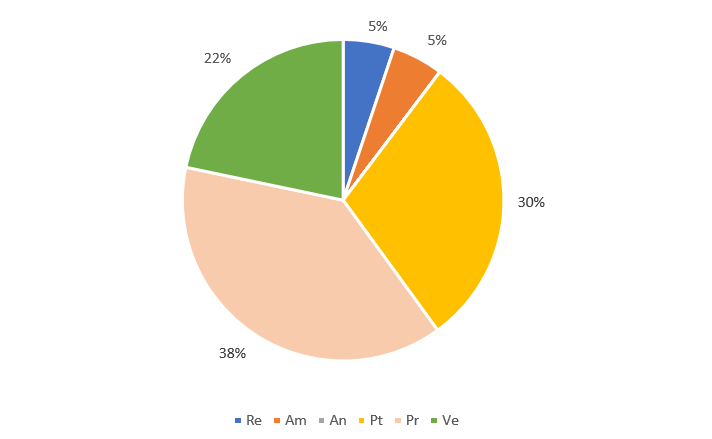
\includegraphics[scale = 0.75]{Immagini/DettaglioTorta.png}
    \caption{Areogramma della ripartizione di ore per ruolo in Progettazione di dettaglio e codifica}
    \label{fig:Areogramma ripartizione ore, periodo di Progettazione di Dettaglio e Codifica}
\end{figure}
\newpage

\subsection{Periodo di Validazione e Collaudo}
\subsubsection{Prospetto orario}
In questo periodo la distribuzione oraria è la seguente:
\begin{table}[H]
	\begin{center}
		\begin{tabular}{ |c c c c c c c c| }
		\rowcolor{darkblue} 
		\textcolor{white}{\textbf{Nominativo}} & \textcolor{white}{\textbf{Re}} & \textcolor{white}{\textbf{Am}} & \textcolor{white}{\textbf{An}} & \textcolor{white}{\textbf{Pt}} & \textcolor{white}{\textbf{Pr}} & \textcolor{white}{\textbf{Ve}} & \textcolor{white}{\textbf{Ore Complessive}} \\ \hline
		\BL 	& -  	& 5  	& - 	& 5 	& - 	& 10 	& 20 \\ \hline
		\FF 	& 4  	& 5  	& - 	& - 	& 5 	& 6  	& 20 \\ \hline
		\MM 	& 4 	& - 	& - 	& - 	& 6 	& 10  	& 20 \\ \hline
		\PC 	& 5 	& -  	& - 	& - 	& 7 	& 8 	& 20 \\ \hline
		\TG 	& -  	& 6 	& - 	& - 	& 8 	& 6 	& 20 \\ \hline
		\TL 	& -  	& - 	& - 	& 4 	& 6 	& 10 	& 20 \\ \hline
		\VD 	& 4  	& -  	& - 	& - 	& 4 	& 12  	& 20 \\ \hline
		\textbf{Ore totali} & \textbf{17} & \textbf{16} & \textbf{-} & \textbf{9} & \textbf{36} & \textbf{62} & \textbf{140} \\ \hline
		\end{tabular}
	\caption{Distribuzione delle ore nel periodo di Validazione e Collaudo}
	\end{center}
\end{table}
I dati ottenuti vengono riassunti nel seguente istogramma:
\begin{figure}[H]
    \centering
    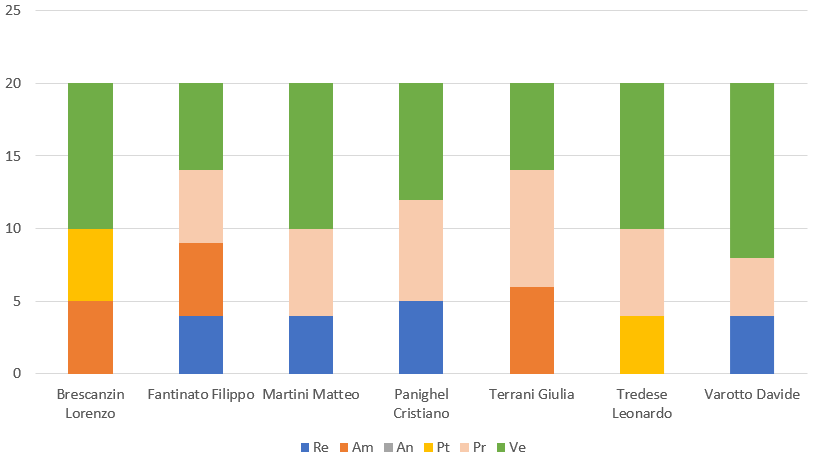
\includegraphics[scale = 0.70]{Immagini/ValidazioneIsto.png}
    \caption{Istogramma della ripartizione delle ore per ruolo in Validazione e collaudo}
    \label{fig:istogramma ripartizione ore, periodo di Validazione e Collaudo}
\end{figure}
\newpage
\subsubsection{Prospetto economico}
Il costo per ogni ruolo è il seguente:
\begin{table}[H]
	\begin{center}
		\begin{tabular}{ |c c c| }
		\rowcolor{darkblue} 
		\textcolor{white}{\textbf{Ruolo}} & \textcolor{white}{\textbf{Ore}} & \textcolor{white}{\textbf{Costo}} \\ \hline
		\textit{\Responsabile} 		& 17 	& 510€ \\ \hline
		\textit{\Amministratore} 	& 16 	& 320€ \\ \hline
		\textit{Analista} 			& - 	& - \\ \hline
		\textit{Progettista} 		& 9 	& 198€ \\ \hline
		\textit{Programmatore}  	& 36 	& 540€ \\ \hline
		\textit{Verificatore} 		& 62 	& 930€ \\ \hline
		\textbf{Totale} & \textbf{140} & \textbf{2498€} \\ \hline
		\end{tabular}
	\caption{ Prospetto dei costi per ruoli nel periodo di Validazione e Collaudo}
	\end{center}
\end{table}
Il seguente grafico a torta riassume i dati ottenuti:
\begin{figure}[H]
    \centering
    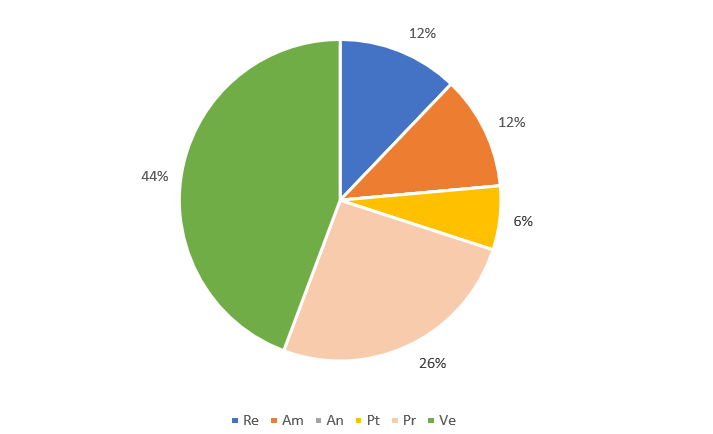
\includegraphics[scale = 0.75]{Immagini/ValidazioneTorta.png}
    \caption{Areogramma della ripartizione di ore per ruolo in Validazione e Collaudo}
    \label{fig:Areogramma ripartizione ore, periodo di Validazione e Collaudo}
\end{figure}
\newpage

\subsection{Riepilogo}
\subsubsection{Ore totali}
\paragraph{Suddivisione del lavoro}
Nella seguente tabella vengono riportate il totale delle ore del progetto, sono presenti sia le ore di investimento, sia le ore rendicontate a carico del committente.
\begin{table}[H]
	\begin{center}
		\begin{tabular}{ |c c c c c c c c| }
		\rowcolor{darkblue} 
		\textcolor{white}{\textbf{Nominativo}} & \textcolor{white}{\textbf{Re}} & \textcolor{white}{\textbf{Am}} & \textcolor{white}{\textbf{An}} & \textcolor{white}{\textbf{Pt}} & \textcolor{white}{\textbf{Pr}} & \textcolor{white}{\textbf{Ve}} & \textcolor{white}{\textbf{Ore Complessive}} \\ \hline
		\BL 	& 4  	& 14  	& 24 	& 35 	& 24 	& 35 	& 136 \\ \hline
		\FF 	& 7 	& 13 	& 18 	& 46 	& 30 	& 22 	& 136 \\ \hline
		\MM 	& 19  	& 11  	& 22 	& 23 	& 26 	& 35  	& 136 \\ \hline
		\PC 	& 15 	& 8  	& 24 	& 13 	& 29	& 47 	& 136 \\ \hline
		\TG 	& 7  	& 26 	& 24 	& 19 	& 28 	& 32 	& 136 \\ \hline
		\TL 	& 12  	& 11 	& 16 	& 19 	& 30 	& 48 	& 136 \\ \hline
		\VD 	& 18  	& 12  	& 16 	& 26 	& 24 	& 40 	& 136 \\ \hline
		\textbf{Ore totali} & \textbf{82} & \textbf{95} & \textbf{144} & \textbf{181} & \textbf{191} & \textbf{259} & \textbf{952} \\ \hline
		\end{tabular}
	\caption{Distribuzione delle ore totali di investimento e rendicontate}
	\end{center}
\end{table}
I dati ottenuti vengono riassunti nel seguente istogramma:
\begin{figure}[H]
    \centering
    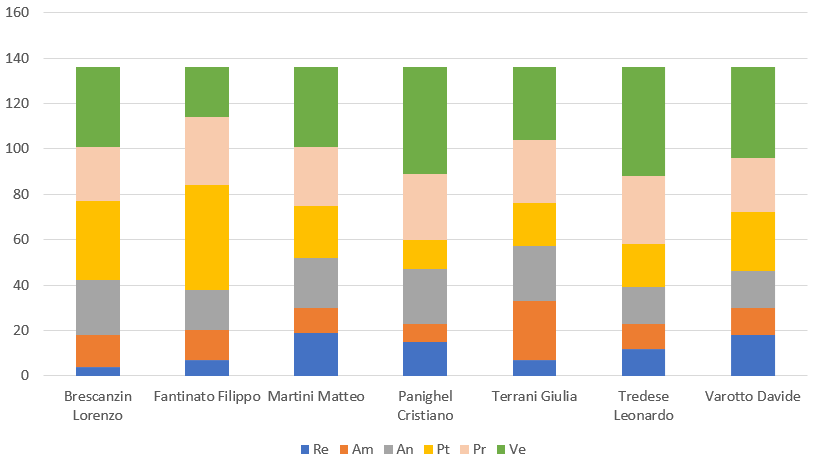
\includegraphics[scale = 0.70]{Immagini/TotaleIsto.png}
    \caption{Istogramma della ripartizione delle ore totali di investimento e rendicontate}
    \label{fig:Istogramma ripartizione ore totali di investimento e rendicontate }
\end{figure}
\newpage
\paragraph{Prospetto economico}
Il costo per ogni ruolo è il seguente:
\begin{table}[H]
	\begin{center}
		\begin{tabular}{ |c c c| }
		\rowcolor{darkblue} 
		\textcolor{white}{\textbf{Ruolo}} & \textcolor{white}{\textbf{Ore}} & \textcolor{white}{\textbf{Costo}} \\ \hline
		\textit{\Responsabile} 		& 82 	& 2460€ \\ \hline
		\textit{\Amministratore} 	& 95 	& 1900€ \\ \hline
		\textit{Analista} 			& 144 	& 3600€ \\ \hline
		\textit{Progettista} 		& 181 	& 3982€ \\ \hline
		\textit{Programmatore}  	& 191 	& 2865€ \\ \hline
		\textit{Verificatore} 		& 259 	& 3885€ \\ \hline
		\textbf{Totale} & \textbf{952} & \textbf{18692€} \\  \hline
		\end{tabular}
	\caption{Prospetto delle ore totali di investimento e rendicontate}
	\end{center}
\end{table}
Il seguente grafico a torta riassume i dati ottenuti:
\begin{figure}[H]
    \centering
    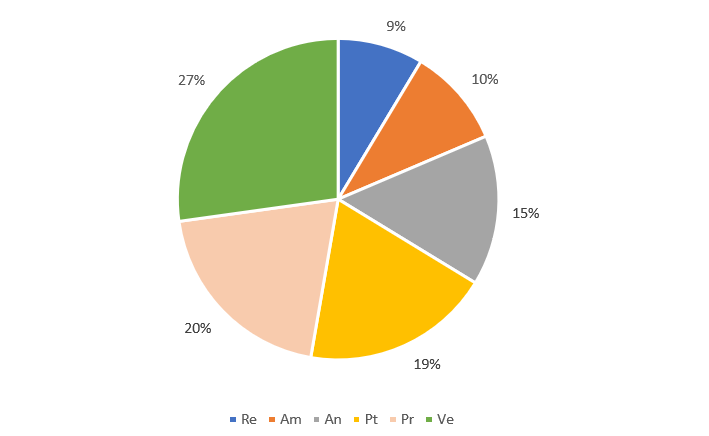
\includegraphics[scale = 0.75]{Immagini/TotaleTorta.png}
    \caption{ Areogramma dei costi totale delle ore di investimento e rendicontate}
    \label{fig:areogramma ripartizione ore totali di investimento e rendicontate}
\end{figure}
\newpage

\subsubsection{Ore rendicontate}
\paragraph{Suddivisione del lavoro}
Nella seguente tabella sono riassunte le ore rendicontate:
\begin{table}[H]
	\begin{center}
		\begin{tabular}{ |c c c c c c c c| }
		\rowcolor{darkblue} 
		\textcolor{white}{\textbf{Nominativo}} & \textcolor{white}{\textbf{Re}} & \textcolor{white}{\textbf{Am}} & \textcolor{white}{\textbf{An}} & \textcolor{white}{\textbf{Pt}} & \textcolor{white}{\textbf{Pr}} & \textcolor{white}{\textbf{Ve}} & \textcolor{white}{\textbf{Ore Complessive}} \\ \hline
		\BL 	& 4  	& 5  	& 8 	& 32 	& 24 	& 27 	& 100 \\ \hline
		\FF 	& 7 	& 5 	& -		& 46 	& 30 	& 12 	& 100 \\ \hline
		\MM 	& 4  	& 11  	& 10 	& 23 	& 26 	& 26  	& 100 \\ \hline
		\PC 	& 10 	& 4  	& 10	& 11 	& 29	& 36 	& 100 \\ \hline
		\TG 	& 5  	& 11 	& 10 	& 19 	& 28 	& 27 	& 100 \\ \hline
		\TL 	& 5  	& 6 	& - 	& 19 	& 32 	& 38 	& 100 \\ \hline
		\VD 	& 18  	& 12  	& -		& 24 	& 24 	& 24 	& 100 \\ \hline
		\textbf{Ore totali} & \textbf{53} & \textbf{54} & \textbf{38} & \textbf{174} & \textbf{191} & \textbf{190} & \textbf{700} \\ \hline
		\end{tabular}
	\caption{Distribuzione delle ore rendicontate}
	\end{center}
\end{table}
I dati ottenuti vengono riassunti nel seguente istogramma:
\begin{figure}[H]
    \centering
    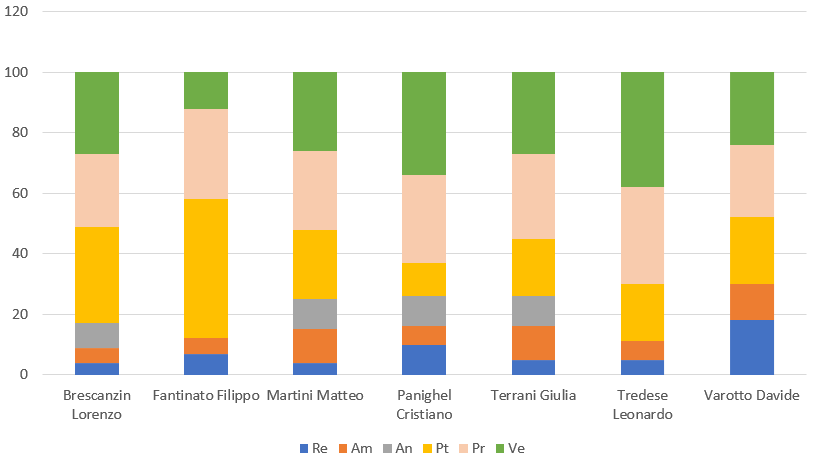
\includegraphics[scale = 0.70]{Immagini/TotaleRendicontatoIsto.png}
    \caption{Istogramma della ripartizione delle ore rendicontate}
    \label{fig:Istogramma ripartizione ore totali rendicontate}
\end{figure}
\newpage
\paragraph{Prospetto economico}
Il costo totale rendicontato per ogni ruolo è il seguente:
\begin{table}[H]
	\begin{center}
		\begin{tabular}{ |c c c| }
		\rowcolor{darkblue} 
		\textcolor{white}{\textbf{Ruolo}} & \textcolor{white}{\textbf{Ore}} & \textcolor{white}{\textbf{Costo}} \\ \hline
		\textit{\Responsabile} 		& 53 	& 1590€ \\ \hline
		\textit{\Amministratore}	& 54 	& 1080€ \\ \hline
		\textit{Analista} 			& 38 	& 950€ \\ \hline
		\textit{Progettista} 		& 174 	& 3828€ \\ \hline
		\textit{Programmatore} 		& 191 	& 2865€ \\ \hline
		\textit{Verificatore} 		& 190 	& 2850€ \\ \hline
		\textbf{Totale} & \textbf{700} & \textbf{13163€} \\ \hline
		\end{tabular}
	\caption{Prospetto delle ore rendicontate}
	\end{center}
\end{table}
Il seguente grafico a torta riassume i dati ottenuti:
\begin{figure}[H]
    \centering
    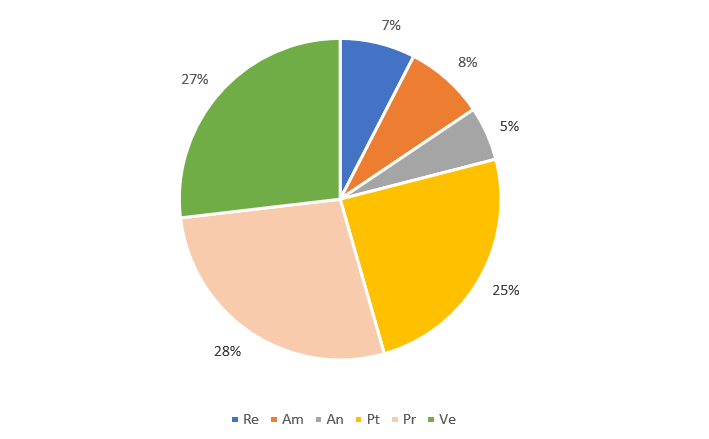
\includegraphics[scale = 0.75]{Immagini/TotaleRendicontatoTorta.png}
    \caption{Areogramma delle ore rendicontate per ruolo}
    \label{fig:Areogramma ripartizione ore totali rendicontate}
\end{figure}
\subsubsection{Conclusioni}
Il costo totale preventivato è: 13163€.
\newpage

\section{Consuntivo e preventivo a finire}
\label{consuntivo_preventivo_a_finire}
Vengono di seguito mostrati i \glo{consuntivi} dei vari periodi con una breve valutazione degli stessi. Sarà inoltre presente un \glo{preventivo} a finire che tiene conto dei soli periodi rendicontati. I valori inseriti nel consuntivo saranno di tue tipologie:
\begin {itemize}
	\item \textbf{Positivi:} se il valore del preventivo è superiore al valore del consuntivo;
	\item \textbf{Negativi:} se il valore del preventivo è inferiore al valore del consuntivo.
\end{itemize}
\subsection{Periodo di Analisi}
L'Analisi è considerata come un periodo di investimento. Il consuntivo viene esposto solamente a scopo informativo e non viene conteggiato nel preventivo a finire.
\subsubsection{Consuntivo}
Di seguito è presente la tabella contenente i dati del consuntivo per il periodo di Analisi.
\begin{table}[H]
	\centering
	\begin{tabular}{|c|c|c|c|c|}
	\rowcolor{darkblue} 
	 	 			&	\multicolumn{2}{c|}{\textcolor{white}{Ore}} 		& 	\multicolumn{2}{c|}{\textcolor{white}{Costo in €}}  \\ \hline
			Ruolo		&	Preventivo	&	Consuntivo	&	Preventivo	&	Consuntivo 	\\ \hline
		Responsabile		&	24		&	24		&	720,00	&	720,00  	\\ \hline
		Amministratore	&	35		&	34 (+1)	&	700,00	&	600,00 (+100,00)  \\ \hline
		Analista		&	89		&	95 (-6)	&	2225,00	&	2375,00 (-150,00)  \\ \hline
		Progettista		& 			&	 		& 			&  			\\ \hline
		Programmatore	& 			& 			& 			&  			\\ \hline
		Verificatore		&	62		&	60 (+2)	&	930,00	&	900,00 (+30,00) 	\\ \hline
		Totale			&	210		&	213		&	4575,00	&	4595,00  	\\ \hline
		Differenza		& 	\multicolumn{2}{c|}{-3 Ore} 	& 	\multicolumn{2}{c|}{-20,00 €} 	\\ \hline
	\end{tabular}
	\caption{Prospetto orario ed economico a consuntivo nella periodo di Analisi}
\end{table}
\subsubsection{Conclusione}
Nello svolgimento dell'attività di analisi si è stati costretti ad impiegare più tempo del previsto per il ruolo di \textit{Analista}, si è invece riusciti a ridurre il consumo di ore nel ruolo di \Amministratore. Questo è dovuto ad una sottostima del carico di lavoro richiesto per la stesura dell'\AdRv{1.0.0}. Il risultato di questo primo periodo è complessivamente di 3 ore lavorative oltre il previsto con una spesa aggiuntiva di 20,00€.
\subsection{Preventivo a finire}
Viene qui mostrata una tabella contenente l'attuale preventivo a finire. I valori relativi all'Analisi e al Consolidamento dei Requisiti sono stati inseriti puramente a scopo riassuntivo. Questi infatti non saranno conteggiati nel calcolo delle ore rendicontate. Se il valore del consuntivo non fosse ancora presente, verrà usato il valore del preventivo.
\begin{table}[H]
	\centering
	\begin{tabular}{|c|c|c|}
	\rowcolor{darkblue} 
		\textcolor{white}{Periodo}	&\textcolor{white}{Preventivo €}	&	\textcolor{white}{Consuntivo €} \\ \hline
		Analisi					&	4575,00				&	4595,00  \\ \hline
		Consolidamento dei requisiti	&	954,00				&	Non presente  \\ \hline
		\rowcolor{darkblue} \multicolumn{3}{|c|}{\textcolor{white}{Rendicontato}}  \\ \hline
		Consolidamento delle tecnologie	&	4327,00				&	Non presente  \\ \hline
		Progettazione e codifica		&	6338,00				&	Non presente  \\ \hline
		Validazione e collaudo		&	2498,00				&	Non presente  \\ \hline
		\rowcolor{darkblue}		&\textcolor{white}{Preventivo €}	&	\textcolor{white}{Preventivo a finire €} \\ \hline
		Totale					&	18692,00				&	18712,00 \\ \hline
		Rendicontato			&	13163,00				&	13183,00 \\ \hline
	\end{tabular}
	\caption{Preventivo a finire - periodo di Analisi}
\end{table}
\newpage

\appendix
\section{Attualizzazione dei rischi}
\label{attualizzazione_dei_rischi}
In questa sezione viene esposto come il gruppo \Gruppo\ ha affrontato le varie problematiche incontrate durante lo svolgimento del progetto.
\subsection{Rischi legati alle tecnologie}
\begin{table} [H]
	\centering
    \begin{tabular}{|c|p{11.5cm}|}
    \rowcolor{darkblue} \hline
    \multicolumn{2}{|c|}{\textcolor{white}{\textbf{RT1 - Inesperienza tecnologica}}}\\ \hline
    Periodo & Analisi.\\ \hline
    Mitigazione & Alcuni membri del gruppo non sono ancora esperti nell'utilizzo di \glo{GitHub} e sono sorti dei leggeri problemi riguardanti la gestione del \glo{repository}. I membri più esperti nell'utilizzo dello strumento hanno dedicato un po' del loro tempo per aiutare i compagni ad imparare a utilizzare al meglio il repository.\\ \hline
	Periodo & Progettazione architetturale.\\ \hline
	Mitigazione & Data la poca esperienza della maggior parte dei componenti del gruppo con le tecnologie da impiegare nello sviluppo del progetto, in particolar modo con \glo{Typescript} e \glo{AWS Lambda}, i membri più esperti nell'utilizzo di queste tecnologie hanno condiviso le loro esperienze con gli altri membri del gruppo. Abbiamo deciso inoltre di dedicare una settimana intera per l'approfondimento individuale.\\ \hline
	\end{tabular}
	\caption{\label{tab:ART1}Attualizzazione dei rischi per inesperienza tecnologica.}
\end{table}
\subsection{Rischi legati ai membri del gruppo}
\begin{table}[H]
	\centering
    \begin{tabular}{|c|p{11.5cm}|}
    \rowcolor{darkblue} \hline
    \multicolumn{2}{|c|}{\textcolor{white}{\textbf{RG3 - Inesperienza gestionale}}}\\ \hline
    Periodo & Analisi.\\ \hline
    Mitigazione & Data l'inesperienza del gruppo nel coordinare il lavoro e alcuni lievi problemi di comunicazione si è verificato un ritardo riguardante la stesura o la verifica. Il gruppo ha cercato di recuperare eventuali mancanze il prima possibile. Essendo in un periodo iniziale del progetto i brevi ritardi verificatosi non hanno causato problemi allo svolgimento del progetto.\\ \hline
    \end{tabular}
    \caption{\label{tab:ARG3}Analisi dei rischi per inesperienza nel coordinamento.}
\end{table}
\begin{table}[H]
	\centering
	\begin{tabular}{|c|p{11.5cm}|}
	\rowcolor{darkblue} \hline
	\multicolumn{2}{|c|}{\textcolor{white}{\textbf{RG2 - Disponibilità dei membri}}}\\ \hline
	Periodo & Progettazione architetturale.\\ \hline
	Mitigazione & La sessione d'esame si è svolta in contemporanea con il periodo di progettazione architetturale e questo ha impegnato notevolmente alcuni membri del gruppo. Per assicurare il procedere del progetto le varie \glo{attività} sono state momentaneamente suddivise tra i membri con maggiori disponibilità.\\ \hline
	\end{tabular}
	\caption{\label{tab:ARG2}Analisi dei rischi per inesperienza nel coordinamento.}
\end{table}
\subsection{Rischi legati ai requisiti}
\begin{table}[H]
	\centering
	\begin{tabular}{|c|p{11.5cm}|}
		\rowcolor{darkblue} \hline
		\multicolumn{2}{|c|}{\textcolor{white}{\textbf{RR1 - Analisi dei requisiti imperfetta}}}\\ \hline
		Periodo & Progettazione architetturale.\\ \hline
		Mitigazione & A seguito delle osservazioni fatte in seguito alla \textbf{Revisione dei Requisiti}, il gruppo {\Gruppo} ha rivisto completamente l'\AdR\ risultata incompleta e con gravi errori di base. Si è provveduto a completare le mancanze segnalate con la massima priorità.\\ \hline
	\end{tabular}
	\caption{\label{tab:ARR1}Analisi dei rischi per analisi dei requisiti imperfetta.}
\end{table}
\newpage

\section{Organigramma}
\label{organigramma}
\subsection{Redazione}
\begin{table}[H]
	\begin{center}
		\begin{tabular}{|c c c|}
			\rowcolor{darkblue}\hline
			\textcolor{white}{Nominativo}&
			\textcolor{white}{Data}&
			\textcolor{white}{Firma}\\ \hline
			\rowcolor{white}
				\TG{} & 2021\_05\_01 & \raisebox{-8pt}{
\includegraphics[height=0.8cm,width=4cm]{Immagini/Firme/FirmaGiulia.jpg}}\\
			\rowcolor{white}
				\FF{} & 2021\_05\_13 & \raisebox{-8pt}{
\includegraphics[height=0.8cm,width=4cm]{Immagini/Firme/FirmaFilippo.jpg}}\\
			\rowcolor{white}
				\BL{} & 2021\_05\_18 & \raisebox{-8pt}{
\includegraphics[height=0.8cm,width=4cm]{Immagini/Firme/FirmaLorenzo.jpg}}\\ \hline
			\rowcolor{white}
		\end{tabular}
	\end{center}
\end{table}
\subsection{Approvazione}
\begin{table}[H]
	\begin{center}
		\begin{tabular}{|c c c|}
			\rowcolor{darkblue}\hline
			\textcolor{white}{Nominativo}&
			\textcolor{white}{Data}&
			\textcolor{white}{Firma}\\ \hline
			\rowcolor{white}
				\PC{} &  2021\_05\_18 & \raisebox{-8pt}{
\includegraphics[height=0.7cm,width=4cm]{Immagini/Firme/FirmaCristiano.jpg}}\\
			\rowcolor{white}
				\VT{} &				& \\
			\rowcolor{white}
				\CR{} &				& \\ \hline
		\end{tabular}
	\end{center}
\end{table}

\subsection{Accettazione dei componenti}
\begin{table}[H]
	\begin{center}
		\begin{tabular}{|c c c|}
			\rowcolor{darkblue}\hline
			\textcolor{white}{Nominativo}&
			\textcolor{white}{Data}&
			\textcolor{white}{Firma}\\ \hline
			\rowcolor{white}
				\BL{} & 2021\_05\_18 & \raisebox{-10pt}{
\includegraphics[scale=0.2]{Immagini/Firme/FirmaLorenzo.jpg}}\\
			\rowcolor{white}
				\FF{} & 2021\_05\_18 & \raisebox{-10pt}{
\includegraphics[scale=0.3]{Immagini/Firme/FirmaFilippo.jpg}}\\
			\rowcolor{white}
				\MM{} & 2021\_05\_18 & \raisebox{-8pt}{
\includegraphics[height=0.8cm,width=4cm]{Immagini/Firme/FirmaMatteo.jpg}}\\
			\rowcolor{white}
				\PC{} & 2021\_05\_18 & \raisebox{-8pt}{
\includegraphics[scale=0.15]{Immagini/Firme/FirmaCristiano.jpg}}\\
			\rowcolor{white}	
				\TG{} & 2021\_05\_18& \raisebox{-10pt}{
\includegraphics[height=0.8cm,width=4cm]{Immagini/Firme/FirmaGiulia.jpg}}\\
			\rowcolor{white}	
				\TL{} & 2021\_05\_18 & \raisebox{-8pt}{
\includegraphics[height=0.7cm,width=4cm]{Immagini/Firme/FirmaLeonardo.jpg}}\\
			\rowcolor{white}	
				\VD{} & 2021\_05\_18 & \raisebox{-8pt}{
\includegraphics[height=0.7cm,width=4cm]{Immagini/Firme/FirmaDavide.jpg}}\\ \hline
		\end{tabular}
	\end{center}
\end{table}

\subsection{Componenti}
\begin{table}[H]%
	\begin{center}
		\begin{tabular}{|c c c|}
			\rowcolor{darkblue}\hline
			\textcolor{white}{Nominativo}&
			\textcolor{white}{Matricola}&
			\textcolor{white}{Indirizzo email}\\ \hline
			\rowcolor{white}
				\BL{} &	1220015	&	lorenzo.brescanzin@studenti.unipd.it\\
			\rowcolor{white}
				\FF{} &	1218816	&	filippo.fantinato.2@studenti.unipd.it\\
			\rowcolor{white}
				\MM{} &	1201150	&	matteo.martini.6@studenti.unipd.it\\
			\rowcolor{white}	
				\PC{} &	1201284	&	cristiano.panighel@studenti.unipd.it\\
			\rowcolor{white}	
				\TG{} &	1142468	&	giulia.terrani@studenti.unipd.it\\
			\rowcolor{white}	
				\TL{} &	1201193	&	leonardo.tredese@studenti.unipd.it\\
			\rowcolor{white}	
				\VD{} &	1201281	& 	davide.varotto.2@studenti.unipd.it\\ \hline
		\end{tabular}
	\end{center}
\end{table}
\end{document}

\end{document}